\documentclass{beamer}
\usepackage[latin1]{inputenc}
\usepackage[3D]{movie15}
%\usetheme{Antibes}
\usetheme{Warsaw}
%\usetheme{Marburg}
%\usetheme[secheader]{Boadilla}
%\usetheme{default}
%\usetheme{Dresden}
%\usetheme{Madrid}
%\usecolortheme{seahorse}
%\usecolortheme{crane}
%\usecolortheme{albatross}
%\usecolortheme{whale}
\usecolortheme{beaver}

\usefonttheme{structuresmallcapsserif}

\title[Anatomical Features]{Multivariate models of inter-subject anatomical variability}
\author{John Ashburner}
\institute[j.ashburner@ucl.ac.uk]{Wellcome Trust Centre for Neuroimaging,\\
UCL Institute of Neurology,\\
12 Queen Square,\\
London WC1N 3BG,\\
UK.}
\date{}
\begin{document}

\begin{frame}
\titlepage
\end{frame}

\section{Introduction}
    \subsection{Why apply pattern recognition to structural MRI?}
    \subsection{Common ways to represent anatomical features}
    \subsection{No Free Lunch and prior knowledge}
    \subsection{Dimensionality reduction}
        \subsubsection{Curse of dimensionality}  \begin{frame}
\frametitle{Curse of dimensionality}
\begin{center}
{\Huge Large $p$, small $n$.\par}
\end{center}
\end{frame}

\begin{frame}
\frametitle{Nearest-neighbour classification}
\begin{columns}[c]
\column{0.7\textwidth}
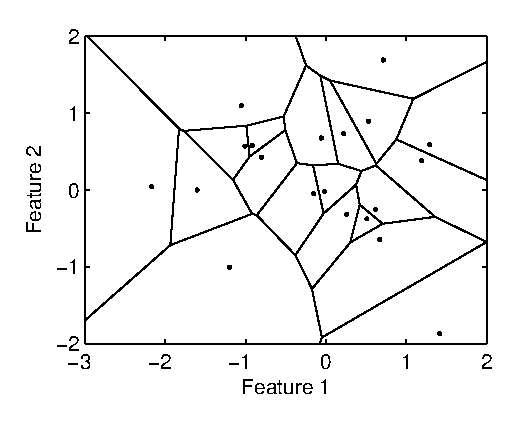
\includegraphics[width=\textwidth]{voronoi}
\column{0.3\textwidth}
\begin{itemize}
\item Not nice smooth separations.
\item Lots of sharp corners.
\item May be improved with \emph{K-nearest neighbours}.
\end{itemize}
\end{columns}
\end{frame}

\begin{frame}
\frametitle{Rule-based approaches}
\begin{columns}[c]
\column{0.7\textwidth}
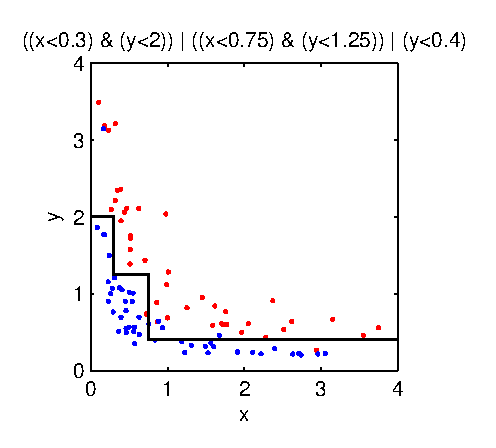
\includegraphics[width=\textwidth]{rule_based}
\column{0.3\textwidth}
\begin{itemize}
\item Not nice smooth separations.
\item Lots of sharp corners.
\end{itemize}
\end{columns}
\end{frame}


\begin{frame}
\frametitle{Corners matter in high-dimensions}
\begin{columns}[c]
\column{0.4\textwidth}
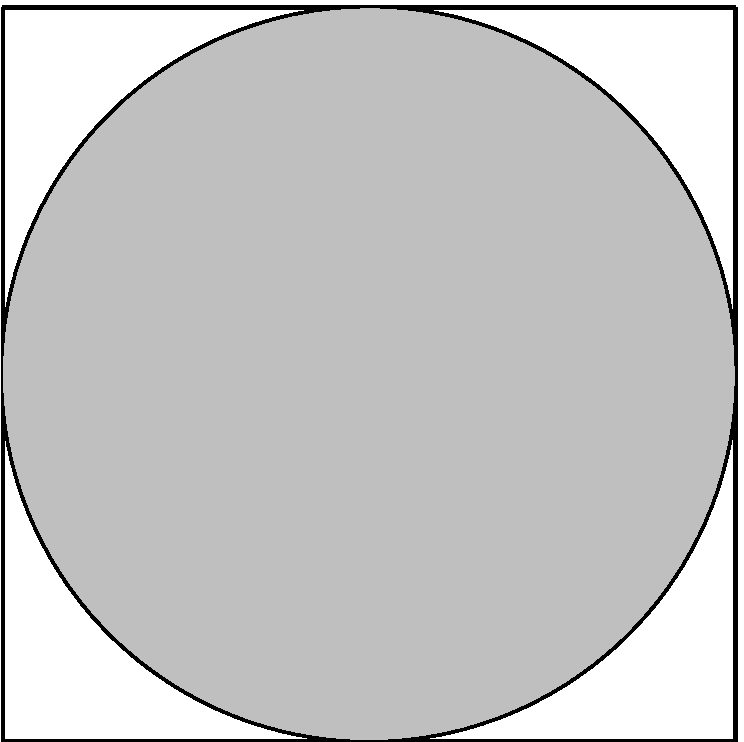
\includegraphics[width=\textwidth]{circle}
\column{0.6\textwidth}
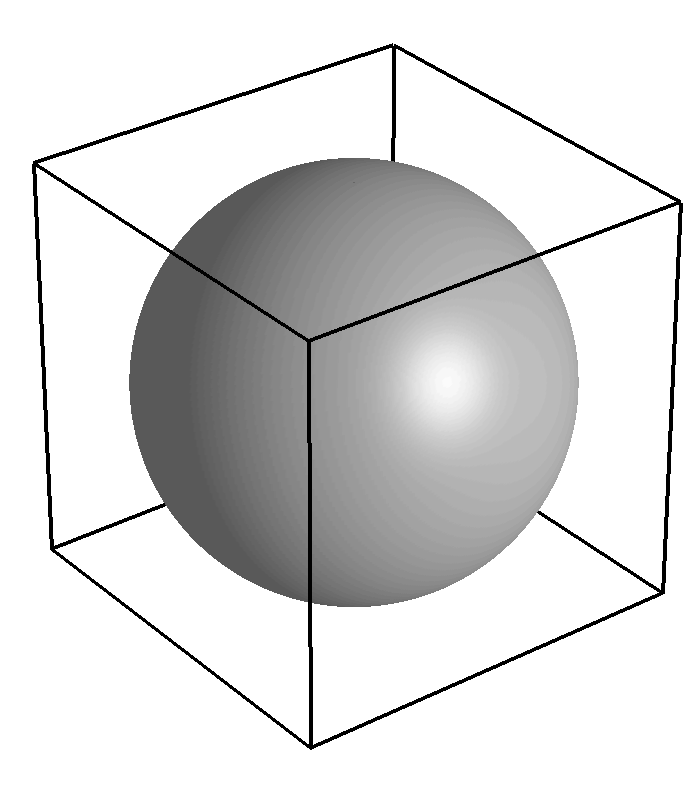
\includegraphics[width=\textwidth]{sphere}
\end{columns}
\end{frame}

\begin{frame}
\frametitle{Corners matter in high-dimensions}
\begin{columns}[c]
\column{0.2\textwidth}
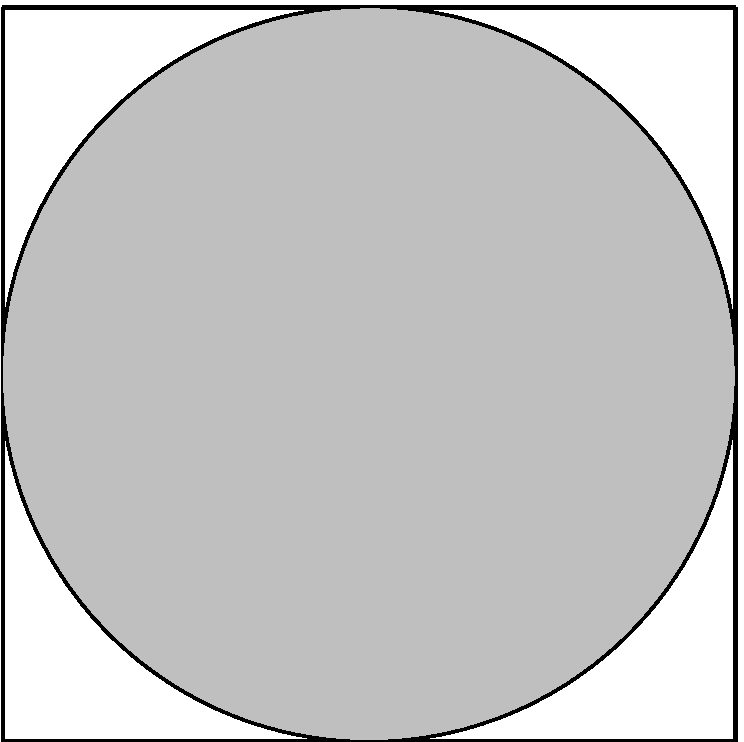
\includegraphics[width=.8\textwidth]{circle}

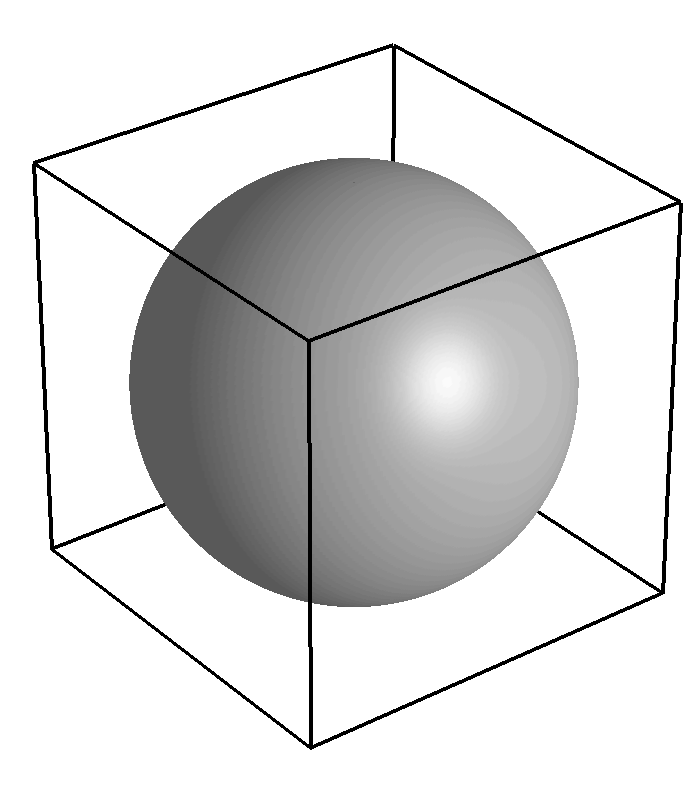
\includegraphics[width=\textwidth]{sphere}
\column{0.8\textwidth}
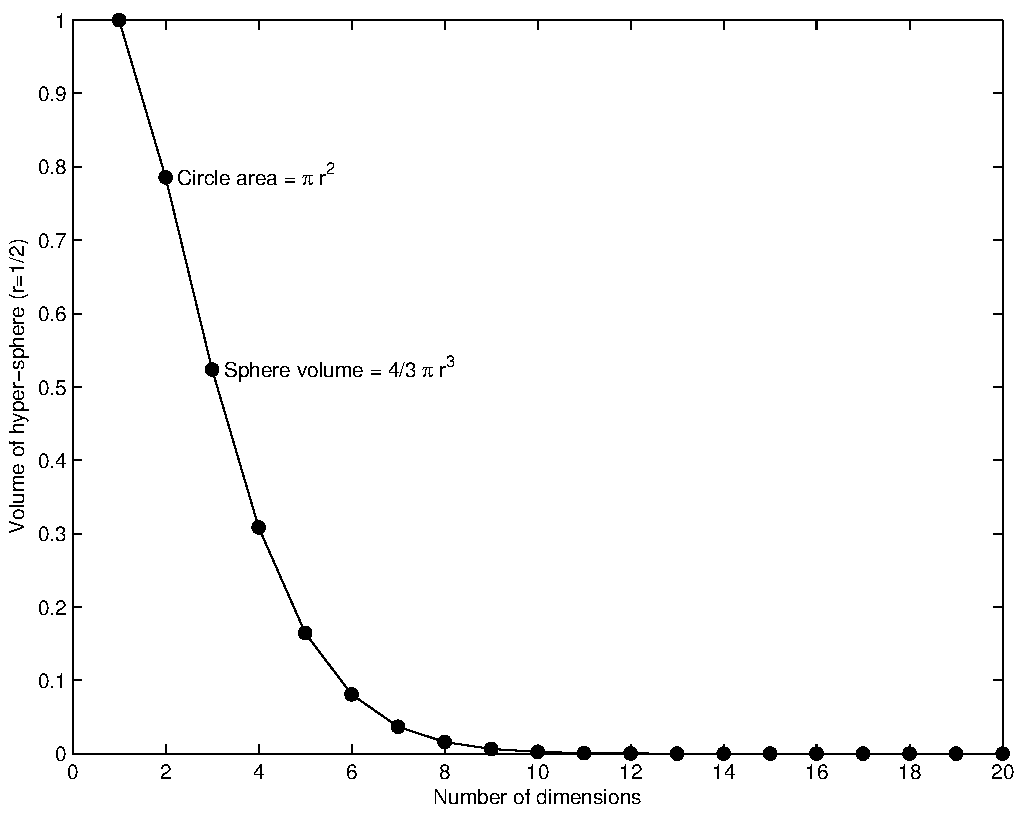
\includegraphics[width=\textwidth]{corners}
\end{columns}
\end{frame}



        \subsubsection{Prediction v Explanation} \begin{frame}
\frametitle{Aims of Science}

\end{frame}


        \subsubsection{Prediction}               \include{Prediction}
        \subsubsection{Binary Classification}    \begin{frame}
\frametitle{A generative classification approach}
\begin{center}
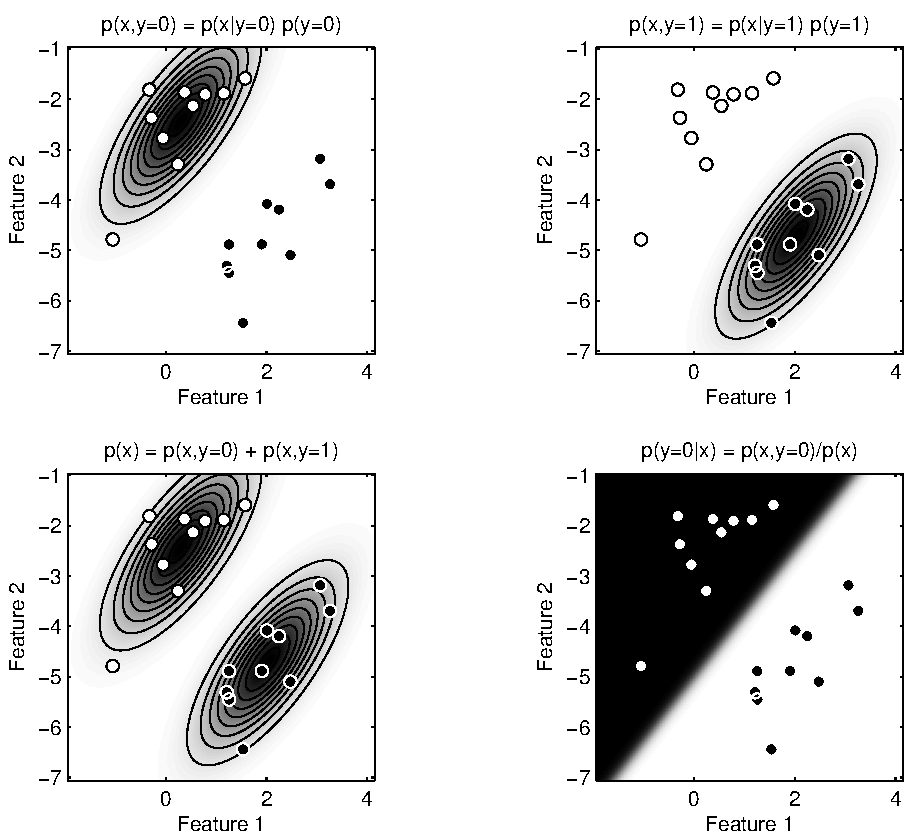
\includegraphics[height=.8\textheight]{fld}
\end{center}
\end{frame}

\begin{frame}
\frametitle{Discriminative classification approaches}
\begin{center}
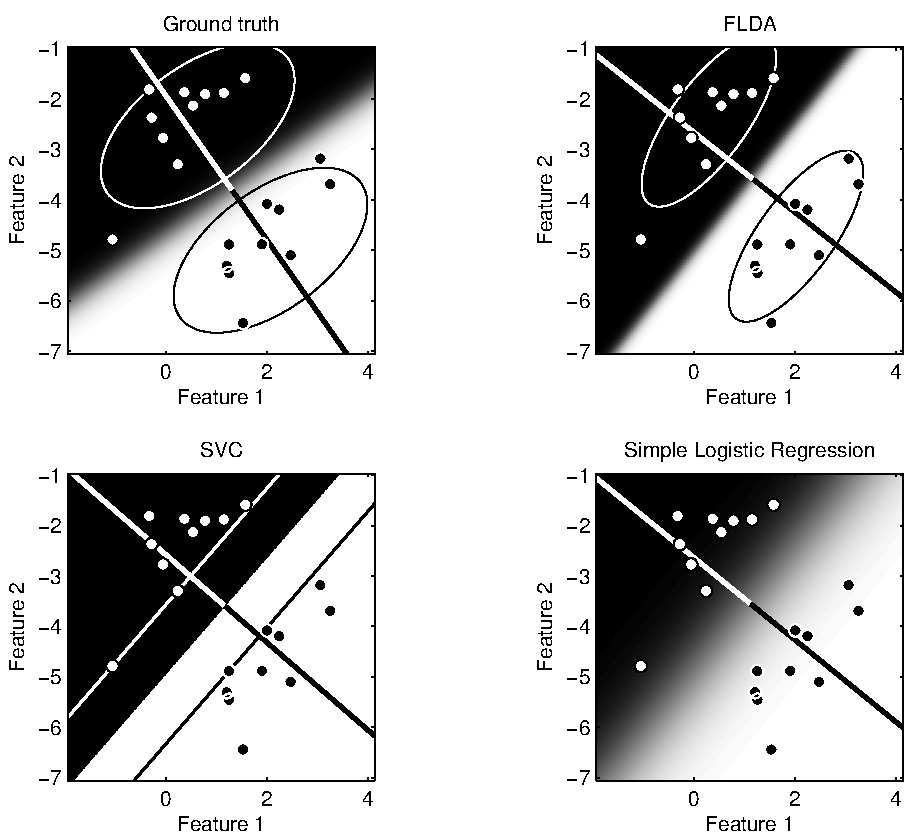
\includegraphics[height=.8\textheight]{linear_discrimination}
\end{center}
\end{frame}

\begin{frame}
\frametitle{Bayesian classification}
\begin{center}
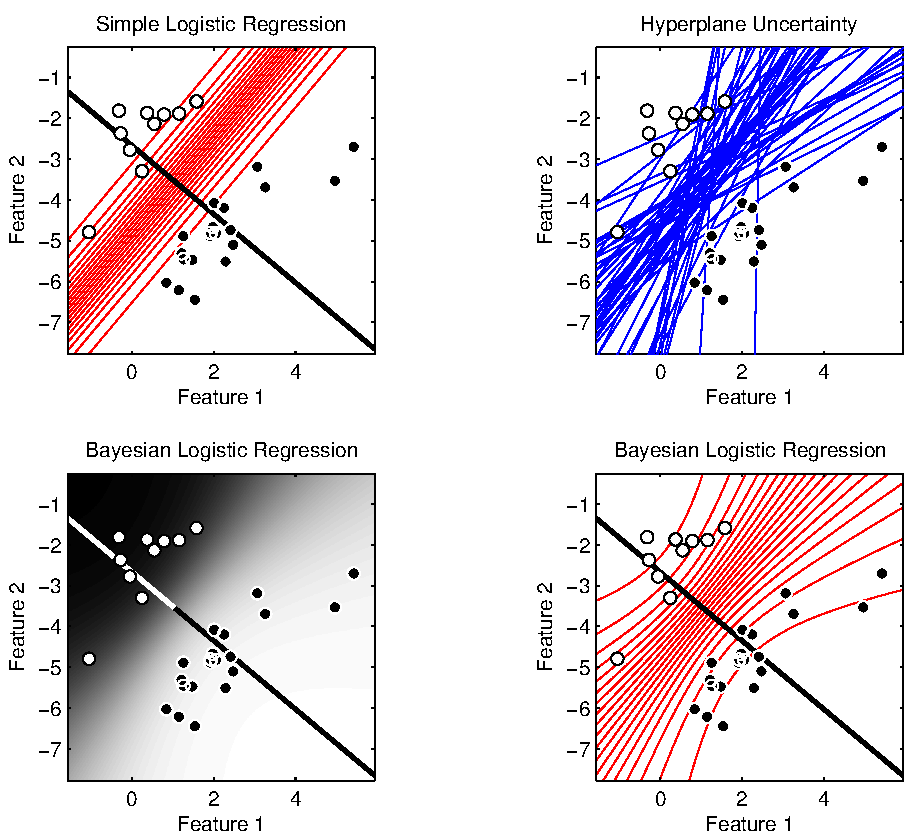
\includegraphics[height=.8\textheight]{logistic_regr}
\end{center}
\end{frame}

\begin{frame}
\frametitle{Why Bayesian?}
\begin{itemize}
\item To deal with different priors.
\begin{itemize}
\item Consider a method with 90\% sensitivity and specificity.
\item Consider using this to screen for a disease afflicting 1\% of the population.
\item On average, out of 100 people there would be 10 wrongly assigned to the disease group.
\item A positive diagnosis suggests only about a 10\% chance of having the disease.
{\small
\begin{eqnarray*}
P(\text{Disease} | \text{Pred+}) & = \frac{P(\text{Pred+} | \text{Disease}) P(\text{Disease})}{P(\text{Pred+} | \text{Disease}) P(\text{Disease}) + P(\text{Pred+} | \text{Healthy}) P(\text{Healthy})}\cr
 & = \frac{\text{Sensitivity} \times P(\text{Disease})}{\text{Sensitivity} \times P(\text{Disease}) + (1-Specificity) \times P(\text{Healthy})}
\end{eqnarray*}
\par
}
\end{itemize}
\item Better decision-making by accounting for utility functions.
\end{itemize}
\end{frame}


        \subsubsection{Kernel methods}           \begin{frame}
\frametitle{Linear regression: maximum likelihood}
A simple way to do regression is by:
\begin{align*}
f({\bf x}_*) = {\bf a}^T {\bf x}_*
\end{align*}
Assuming Gaussian noise on ${\bf y}$, the ML estimate of ${\bf a}$ is by:
\begin{align*}
\hat{\bf a} = ({\bf X}^T{\bf X})^{-1}{\bf X}^T {\bf y}
\end{align*}
where
\begin{align*}
{\bf X} = \begin{pmatrix}{\bf x}_1 & {\bf x}_2 & \hdots & {\bf x}_n\end{pmatrix}^T \text{, and }
{\bf y} = \begin{pmatrix}y_1 & y_2 & \hdots y_n\end{pmatrix}^T
\end{align*}
Model has $p$ parameters to estimate.\par
Number of observations is $n$ (number of targets).\par
Usualy needs dimensionality reduction, with (eg) SVD.
\end{frame}

\begin{frame}
\frametitle{Linear regression: maximum posterior}
We may have prior knowledge about various distributions:
\begin{align*}
p(y_* | {\bf x}_*, {\bf a}) = & \mathcal{N}({\bf a}^T{\bf x}_*, \sigma^2)\cr
p({\bf a}) = & \mathcal{N}({\bf 0},\boldsymbol\Sigma_0)\cr
\end{align*}
Therefore,
\begin{align*}
p({\bf a}|{\bf y},{\bf X})  = & \mathcal{N}(\sigma^{-2}{\bf B}^{-1}{\bf X}^T{\bf y},{\bf B}^{-1}) \text{, where } {\bf B} = \sigma^{-2}{\bf X}^T{\bf X} + \boldsymbol\Sigma_0^{-1}
\end{align*}

Maximum a posteriori (MAP) estimate of ${\bf a}$ is by:
\begin{align*}
\hat{\bf a} = \sigma^{-2}{\bf B}^{-1}{\bf X}^T{\bf y} \text{, where } {\bf B} = \sigma^{-2}{\bf X}^T{\bf X} + \boldsymbol\Sigma_0^{-1}
\end{align*}
\end{frame}

\begin{frame}
\frametitle{Linear regression: Bayesian}
We may have prior knowledge about various distributions:
\begin{align*}
p(y_* | {\bf x}_*, {\bf a}) = & \mathcal{N}({\bf a}^T{\bf x}_*, \sigma^2)\cr
p({\bf a}) = & \mathcal{N}({\bf 0},\boldsymbol\Sigma_0)\cr
\end{align*}
Therefore,
\begin{align*}
p({\bf a}|{\bf y},{\bf X})  = & \mathcal{N}(\sigma^{-2}{\bf B}^{-1}{\bf X}^T{\bf y},{\bf B}^{-1}) \text{, where } {\bf B} = \sigma^{-2}{\bf X}^T{\bf X} + \boldsymbol\Sigma_0^{-1}
\end{align*}
Predictions are made by integrating out the uncertainty of the weights, rather than estimating them:
\begin{align*}
p(y_* | {\bf x}_*, {\bf y}, {\bf X}) = & \int_{\bf a} p(y_* | {\bf x}_*, {\bf a}) p({\bf a}|{\bf y},{\bf X}) d{\bf a}\cr
                                     = & \mathcal{N}(\sigma^{-2} {\bf x}_*^T {\bf B}^{-1} {\bf X}^T {\bf y}, {\bf x}_*^T{\bf B}^{-1}{\bf x}_*)
\end{align*}
Estimated parameters may be $\sigma^2$, and parameters encoding $\boldsymbol\Sigma_0$.
\end{frame}

\begin{frame}
\frametitle{Kernel methods: Woodbury matrix identity}
\begin{align*}
{\bf B}^{-1} = & \left(\sigma^{-2}{\bf X}^T{\bf X} + \boldsymbol\Sigma_0^{-1}\right)^{-1}\\
             = & \boldsymbol\Sigma_0 - \boldsymbol\Sigma_0 {\bf X}^T({\bf I}\sigma^2 + {\bf X} \boldsymbol\Sigma_0 {\bf X}^T)^{-1} {\bf X} \boldsymbol\Sigma_0
\end{align*}

\vspace{0.25cm}
\begin{tiny}
Wikipedia contributors, ``Woodbury matrix identity,'' Wikipedia, The Free Encyclopedia, \url{http://en.wikipedia.org/w/index.php?title=Woodbury\_matrix\_identity\&oldid=638370219} (accessed April 1, 2015).\par
\end{tiny}
Dimensions of ${\bf X}^T{\bf X}$ are $p \times p$.\par
Dimensions of ${\bf X} \boldsymbol\Sigma_0 {\bf X}^T$ are $n \times n$.\par
\end{frame}

\begin{frame}
\frametitle{Kernel methods: Gaussian process regression}
The predicted distribution is:
\begin{align*}
p(y_*|{\bf x}_*,{\bf y},{\bf X}) = &\mathcal{N}({\bf k}^T{\bf C}^{-1} {\bf y},c - {\bf k}^T {\bf C}^{-1} {\bf k})
\end{align*}
where:
\begin{align*}
{\bf C} = & {\bf X} \boldsymbol\Sigma_0 {\bf X}^T + {\bf I}\sigma^2\\
{\bf k} = & {\bf X} \boldsymbol\Sigma_0 {\bf x}_*\\
c = & {\bf x}_*^T \boldsymbol\Sigma_0 {\bf x}_* + \sigma^2
\end{align*}
\end{frame}

\begin{frame}
\frametitle{Kernel methods: nonlinear methods}
%\begin{columns}[c]
%\column{0.5\textwidth}
Sometimes, we want alternatives to ${\bf C} = {\bf X} \boldsymbol\Sigma_0 {\bf X}^T + {\bf I}\sigma^2$.\par
Nonlinearity is achieved by replacing the matrix ${\bf K} = {\bf X} \boldsymbol\Sigma_0 {\bf X}^T$ with some function of the data that gives a positive definite matrix encoding similarities.\par
eg
\begin{align*}
k({\bf x}_i,{\bf x}_j) = \theta_1 + \theta_2 {\bf x}_i \cdot {\bf x_j} + \theta_3 \exp\left(-\frac{||{\bf x}_i - {\bf x_j}||^2}{2 \theta_4^2}\right)
\end{align*}

Hyper-parameters $\theta_1$ to $\theta_4$ can be optimised in a number of ways.\par
%\column{0.5\textwidth}
%Examples include:
%\begin{itemize}
%\item Linear: $k({\bf x}_i,{\bf x}_j) = {\bf x}_i \cdot {\bf x}_k$
%\item 
%\end{itemize}
%\includegraphics[width=.75\textwidth]{nonlinear_kernels}
%\end{columns}
\end{frame}

\begin{frame}
\frametitle{Kernel methods: nonlinear methods}
\begin{columns}[cc]
\column{0.6\textwidth}
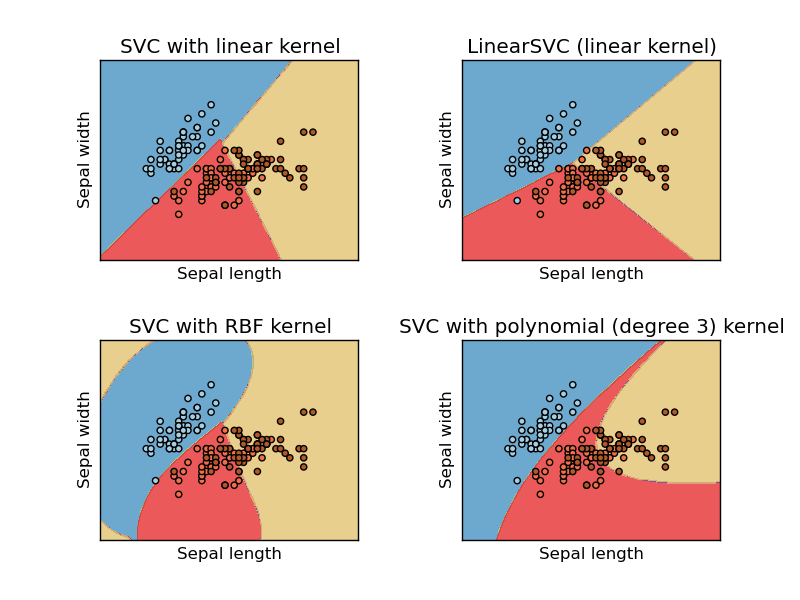
\includegraphics[width=\textwidth]{sklearn_material/plot_iris_0012.png}
\column{0.4\textwidth} Non-linear methods are useful in low-dimension
to adapt the shape of decision boundaries.
\end{columns}
For large $p$, small $n$ problems, nonlinear methods do not seem to help much.\par
Nonlinearity also reduces interpretability.
\end{frame}

\begin{frame}
\frametitle{Discriminative models for classification}
\begin{columns}[c]
\column{0.5\textwidth}
\begin{align*}
t = \sigma(f({\bf x}_*)) 
\end{align*}
where $\sigma$ is some squashing function, eg:
\begin{itemize}
\item Heaviside step function.
\item Logistic function (inverse of Logit).
\item Normal CDF (inverse of Probit).
\item Hinge loss (support vector machines)
\end{itemize}
\column{0.5\textwidth}
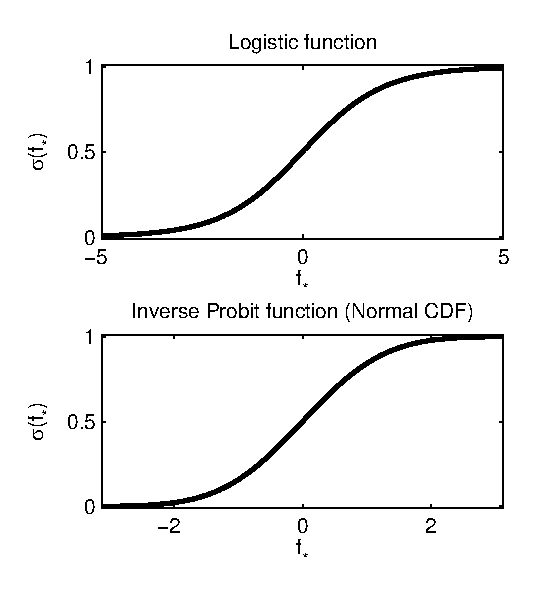
\includegraphics[width=.75\textwidth]{squashing}

\textbf{Bertrand: maybe a distinction should be introduced here between the decision function (typically the sign function) and the loss function used for training.}

\end{columns}
\end{frame}

\begin{frame}
\frametitle{Discriminative models for classification: convexity} 

In practice, the hinge and logistic losses yield a convex estimation
problem and are preferred.

\begin{align*}
\text{min}_{\mathbf{w}} \; \sum_{i=1}^n \mathcal{L}(y_i,\mathbf{X_i},\mathbf{w}) + \lambda \mathcal{R} (\mathbf{w})
\end{align*}


(M-estimators framework)
\begin{itemize}
\item $\mathcal{L}$ is the loss function (hinge, logistic, quadratic...)
\item $\mathcal{R}$ is the regularizer (typically a norm on $\mathbf{w}$) 
\item $\lambda > 0$ balances the two terms
\end{itemize}
$\mathcal{L}$ and $\mathcal{R}$ convex $\rightarrow$ unique minimizer (SVMs, $\ell_2$-logistic, $\ell_1$-logistic).

\end{frame}

\begin{frame}
\frametitle{Probabilistic classification}
\begin{columns}[c]
\column{0.5\textwidth}
Integrating over the uncertainty of the separating hyperplane allows probabilistic predictions further from the training data.\par
This is not usually done for methods such as the relevance-vector machine (RVM).\par
\vspace{0.25cm}
\begin{tiny}
Rasmussen, Carl Edward, and Joaquin Quinonero-Candela. ``Healing the relevance vector machine through augmentation.'' In Proceedings of the 22nd international conference on Machine learning, pp. 689-696. ACM, 2005.\par
\end{tiny}
\column{0.5\textwidth}
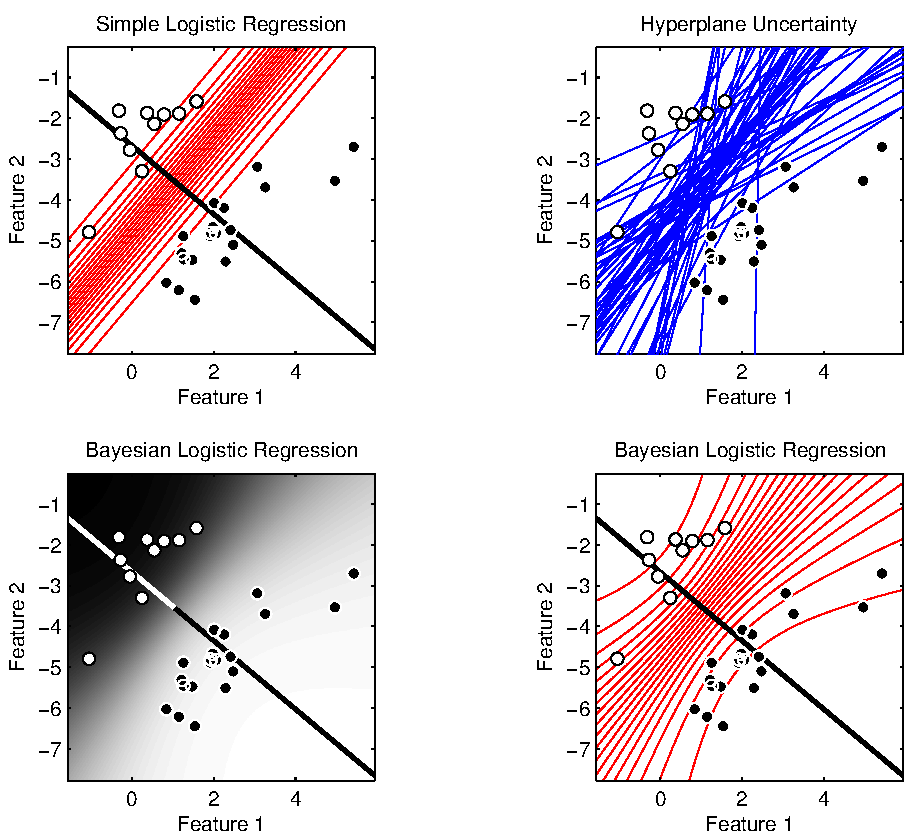
\includegraphics[width=\textwidth]{logistic_regr}
\end{columns}
\end{frame}

\begin{frame}
\frametitle{Probabilistic classification}
Making probabilistic predictions involves:
\begin{enumerate}
\item Computing the distribution of a latent variable corresponding to the test data (cf regression):
\begin{align*}
p(f_* | {\bf x}_*, {\bf y}, {\bf X}) = & \int_{\bf f} p(f_* | {\bf x}_*, {\bf f}) p({\bf f}|{\bf y},{\bf X}) d{\bf f}
\end{align*}
\item Using this distribution to give a probabilistic prediction:
\begin{align*}
P(y_*=1|{\bf x}_*,{\bf y},{\bf X}) = \int_{f_*} \sigma(f_*) p(f_*|{\bf x}_*,{\bf y},{\bf X}) df_*
\end{align*}
\end{enumerate}
Unfortunately, the second integral is analytically intractable, so approximations are needed.\par
\end{frame}

\begin{frame}
\frametitle{Probabilistic classification}
Approximate methods for probabilistic classification include:
\begin{itemize}
\item {\bf The Laplace Approximation} (LA).  Fastest, but less accurate.
\item {\bf Expectation Propagation} (EP).  More accurate than the Laplace approximation, but slightly slower.
\item {\bf MCMC} methods. The ``gold standard'', but very slow to draw lots of random samples.
\end{itemize}
\vspace{0.25cm}
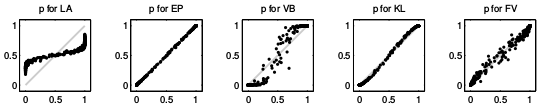
\includegraphics[width=\textwidth]{nickisch_figure}
\begin{tiny}
Nickisch, Hannes, and Carl Edward Rasmussen. ``Approximations for Binary Gaussian Process Classification.'' Journal of Machine Learning Research 9 (2008): 2035-2078.\par
\end{tiny}
\end{frame}

\begin{frame}
\frametitle{Support vector classification}
\begin{columns}[c]
\column{0.5\textwidth}
If you are only interested in binary predictions, support-vector machines are reasonably fast and accurate.\par
%Targets are ${\bf t} \in \{-1,1\}$.\\
%Solves a quadratic programming problem
%\begin{align*}
%\hat{\boldsymbol\alpha} = \argmin_{\boldsymbol\alpha} \tfrac{1}{2} {\boldsymbol\alpha}^T {\bf H}{\boldsymbol\alpha} - \sum_{i=1}^n \alpha_i,\\
%\text{subject to }
%{\bf t}^T{\boldsymbol\alpha} = 0 \text{ and }
%0 \le \alpha_i \le C\\
%\text{where }
%{\bf H} = \diag({\bf t}) {\bf X}{\bf X}^T \diag({\bf t})
%\end{align*}
%Binary prediction is by:
%\begin{align*}
%t_* = sgn(\sum_{i=1}^N t_i \alpha_i {\bf x}_i {\bf x}_*^T + b)
%\end{align*}
%where $b$ is a bias term.
\column{0.5\textwidth}
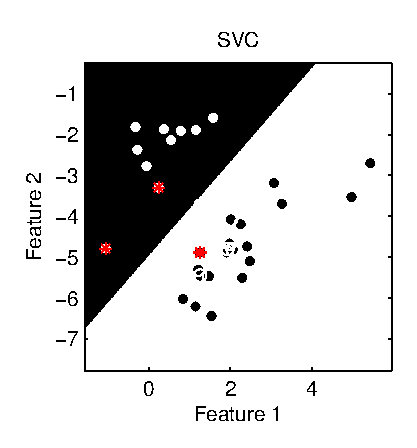
\includegraphics[width=\textwidth]{svc}
\end{columns}
\end{frame}



\section{Geometric Morphometrics}
    \subsection{Early univariate morphometry}
    \subsection{Early multivariate morphometry}
    \subsection{The morphometrics ``revolution'' (landmarks)}
    \subsection{Allometric relations}
    \subsection{Automated shape estimation}

    %\subsection{Geometric Variability}
        \subsubsection{Principal Components}     \begin{frame}
\frametitle{One mode of geometric variability}
\begin{columns}[c]
\column{0.5\textwidth}
Simulated images\par
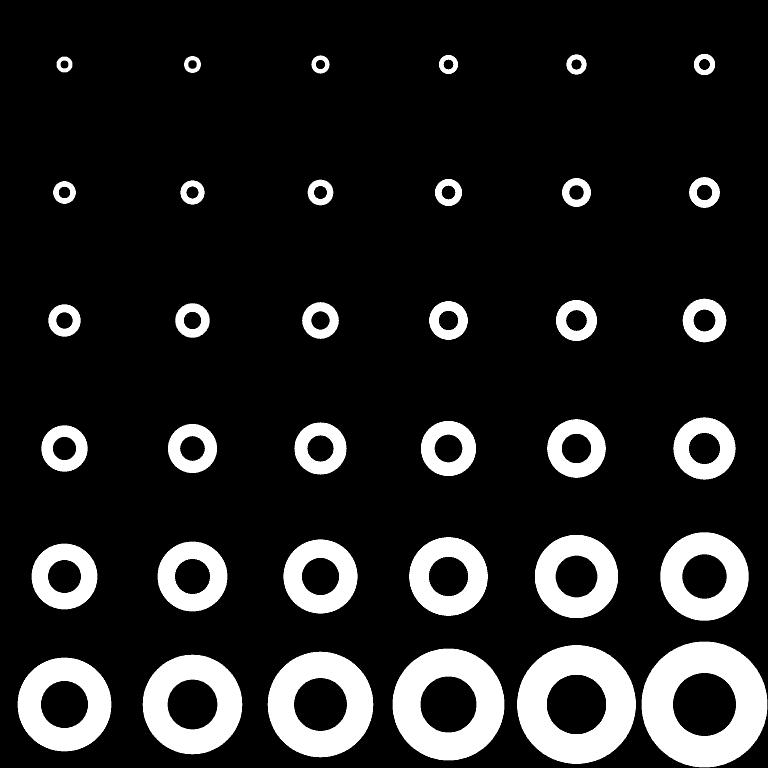
\includegraphics[height=0.9\textwidth]{circles}
\column{0.5\textwidth}
Principal components\par
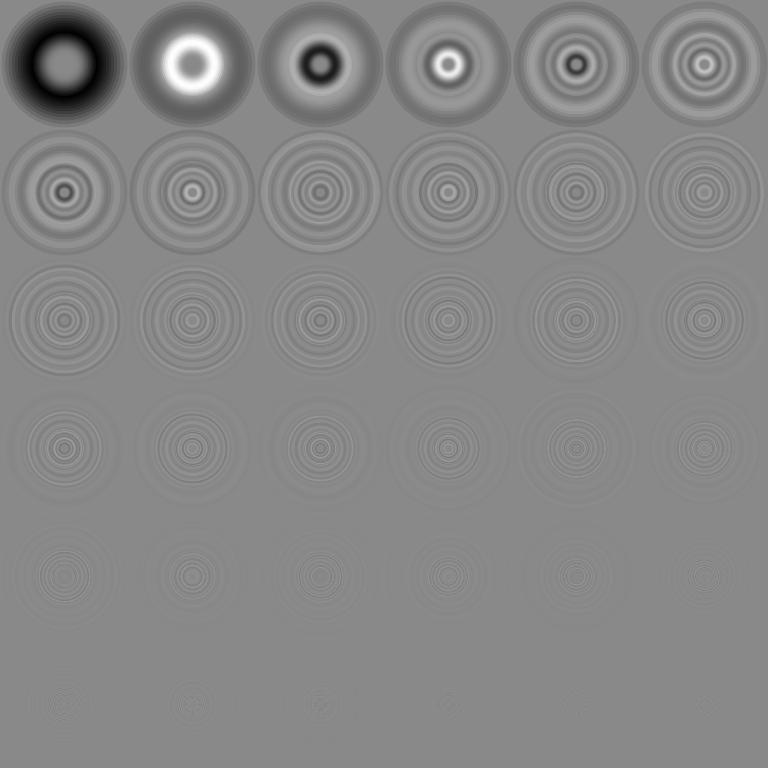
\includegraphics[height=0.9\textwidth]{circles_pca}
\end{columns}
A suitable model would reduce these data to a single dimension.
\end{frame}


\begin{frame}
\frametitle{Two modes of geometric variability}
\begin{columns}[c]
\column{0.5\textwidth}
Simulated images\par
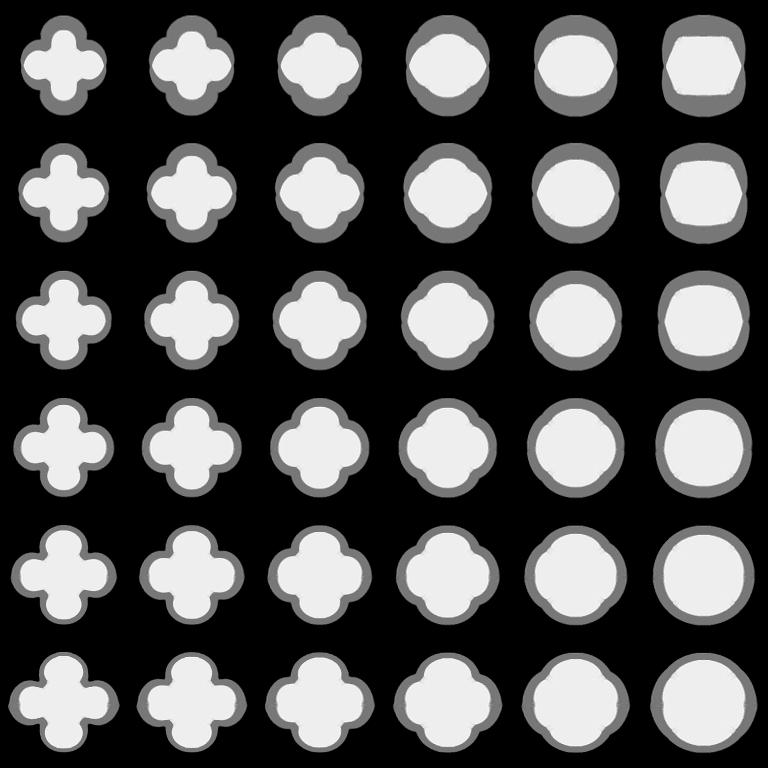
\includegraphics[height=0.9\textwidth]{things}
\column{0.5\textwidth}
Principal components\par
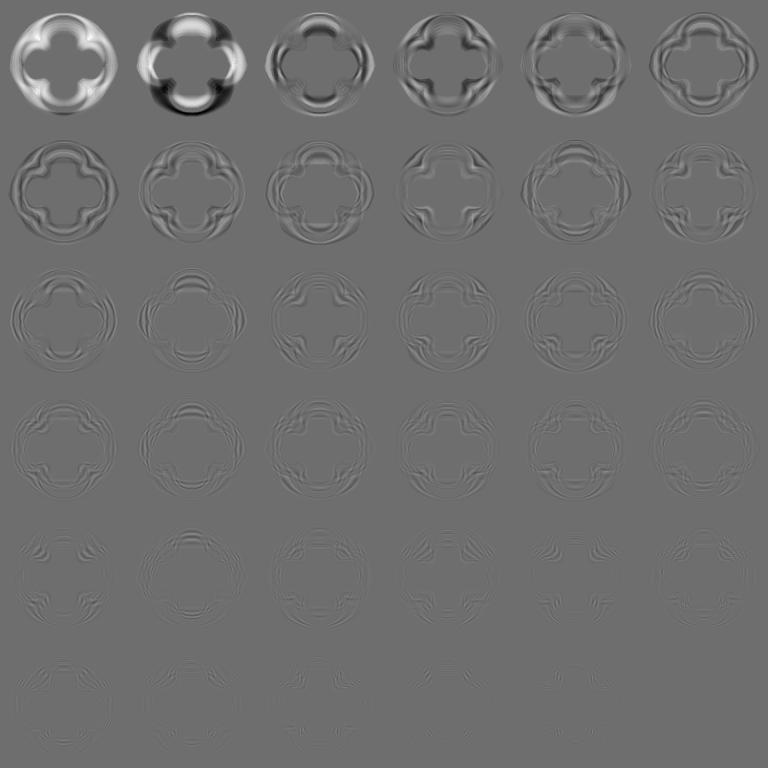
\includegraphics[height=0.9\textwidth]{things_pca}
\end{columns}
A suitable model would reduce these data to two dimensions.
\end{frame}



\section{Similarity between brains}
    \subsection{Distances between anatomies} \begin{frame}
\frametitle{Similarity Measures}
\begin{itemize}
\item Many methods are based on similarity measures.
\item A common similarity measure is the dot product.
\begin{eqnarray*}
\text{Similarity: } k({\bf x},{\bf y}) = \sum_k x_k y_k
\end{eqnarray*}
\item Nonlinear methods are often based on distances.
\begin{eqnarray*}
\text{Distance: } & d({\bf x},{\bf y}) = & \sqrt{\sum_k (x_k-y_k)^2}\cr
\text{Similarity: } & k({\bf x},{\bf y}) = & exp(-\lambda d({\bf x},{\bf y})^2)
\end{eqnarray*}
\item How do we best measure distances between brain images?
\end{itemize}
\end{frame}

%\begin{frame}
%\frametitle{No Free Ducklings}
%{\bf No Free Lunch theorem} says that learning is impossible without prior knowledge (\url{http://en.wikipedia.org/wiki/No\_free\_lunch\_in\_search\_and\_optimization}).

%{\bf Ugly Duckling theorem} says that things are all equivalently similar to each other without prior knowledge (\url{http://en.wikipedia.org/wiki/Ugly\_duckling\_theorem}).

%\vspace{1cm}
%What prior knowledge do we have about the variability among people that can be measured using MRI?

%How do we use this knowledge?
%\end{frame}

\begin{frame}
\frametitle{Image Registration}
\begin{columns}[c]
\column{0.7\textwidth}
\begin{itemize}
\item Image registration measures distances between images.
\item Often involves minimising the sum of two terms:
\begin{itemize}
\item Distance between the image intensities.
\item Distance of the deformation from zero.
\end{itemize}
\item The sum of these terms gives the distance.
\end{itemize}
\column{0.3\textwidth}
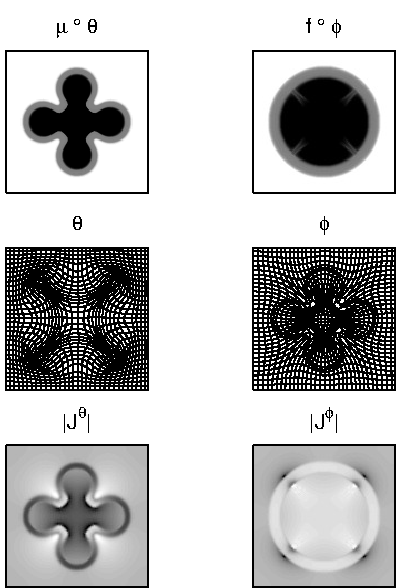
\includegraphics[width=\textwidth]{shoot2d}
\end{columns}
\end{frame}

\begin{frame}
\frametitle{Different ways of measuring distances}
\begin{columns}[c]
\column{.3\textwidth}
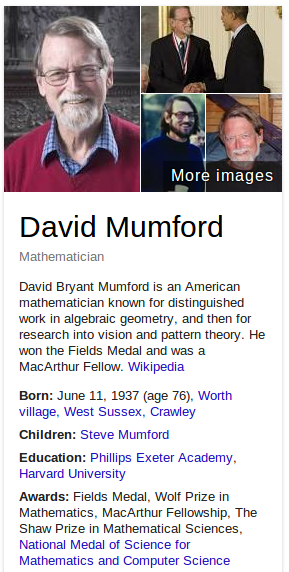
\includegraphics[width=\textwidth]{mumford}
\column{.7\textwidth}
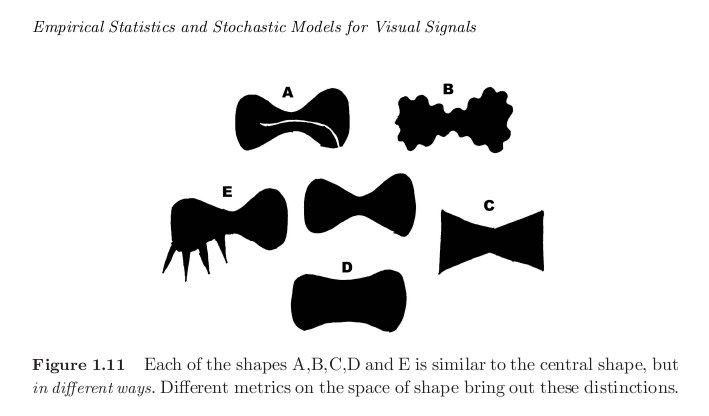
\includegraphics[width=\textwidth]{mumford_fig}
\end{columns}
\end{frame}

\begin{frame}
\frametitle{Different ways of measuring distances}
\begin{columns}[c]
\column{.2\textwidth}
\begin{center}
Two simulated images\par
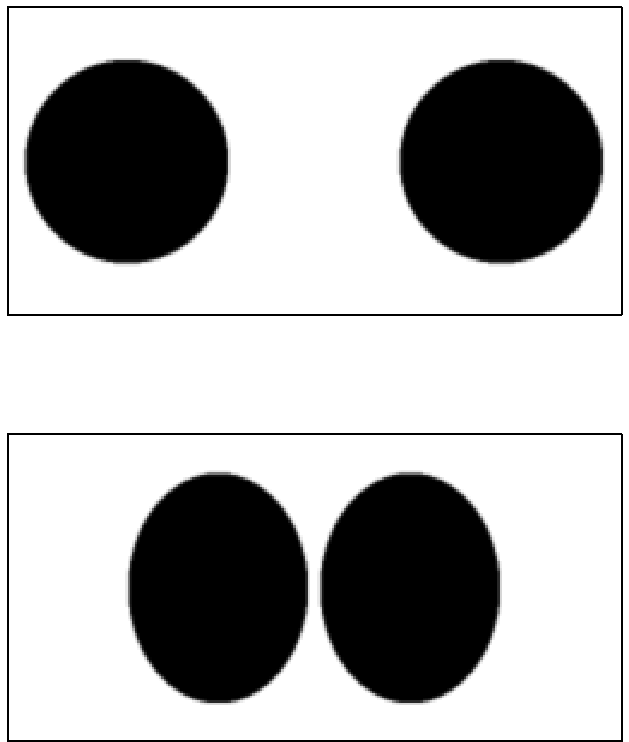
\includegraphics[width=\textwidth]{figure2Di}
\end{center}
\column{.8\textwidth}
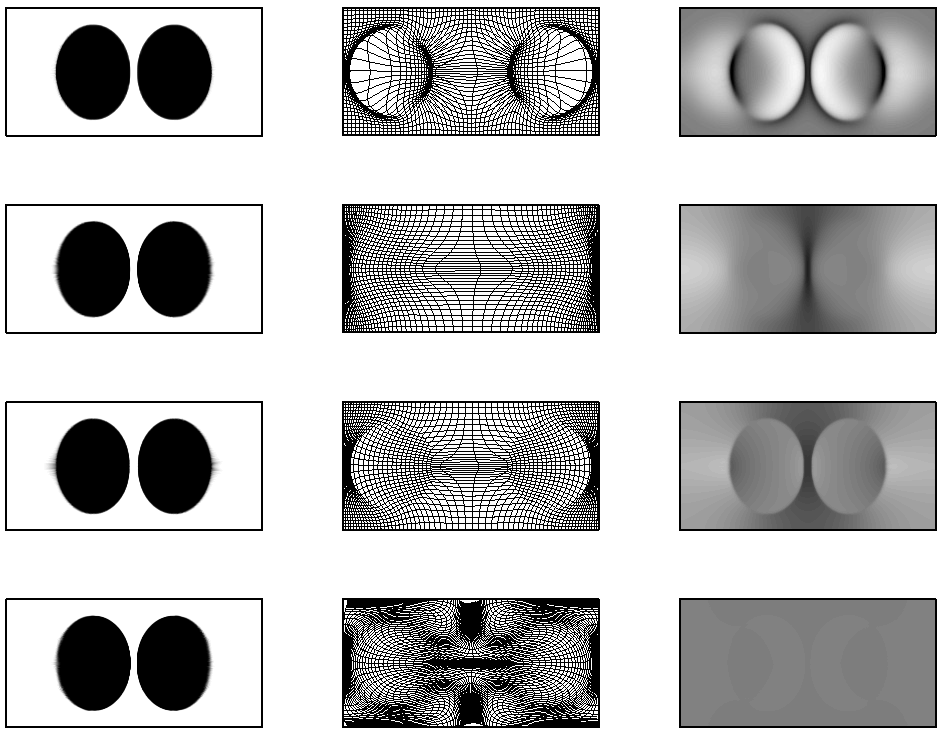
\includegraphics[width=\textwidth]{figure2Dii}
\end{columns}
\end{frame}

\begin{frame}
\frametitle{Metrics}
Distances need to satisfy the properties of a \emph{metric}:
\begin{enumerate}
\item $d({\bf x}, {\bf y}) \ge 0$ (non-negativity)
\item $d({\bf x}, {\bf y}) = 0$ if and only if ${\bf x} = {\bf y}$ (identity of indiscernibles)
\item $d({\bf x}, {\bf y}) = d({\bf y}, {\bf x})$ (symmetry)
\item $d({\bf x}, {\bf z}) \le d({\bf x}, {\bf y}) + d({\bf y}, {\bf z})$ (triangle inequality).
\end{enumerate}

Satisfying (3) requires inverse-consistent image registration.

Satisfying (4) requires a specific class of image registration models.
\end{frame}


\begin{frame}
\frametitle{Non-Euclidean geometry}
\begin{columns}[c]
\column{0.5\textwidth}
\begin{itemize}
\item Distances are not always measured along a straight line.
\item ``\emph{Shapes are the ultimate non-linear sort of thing}''
\end{itemize}
\column{0.5\textwidth}
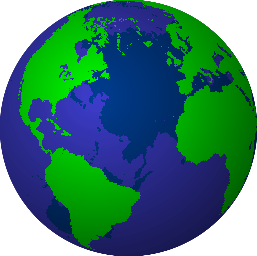
\includegraphics[width=\textwidth]{Globe}
\end{columns}
\end{frame}

\begin{frame}
\frametitle{Linear approximations to nonlinear problems}
%\begin{columns}[c]
%\column{0.2\textwidth}
%Dealing with non-Euclidean geometry.
%Linear approximation around the average.
%\begin{center}
%\column{0.8\textwidth}
\begin{center}
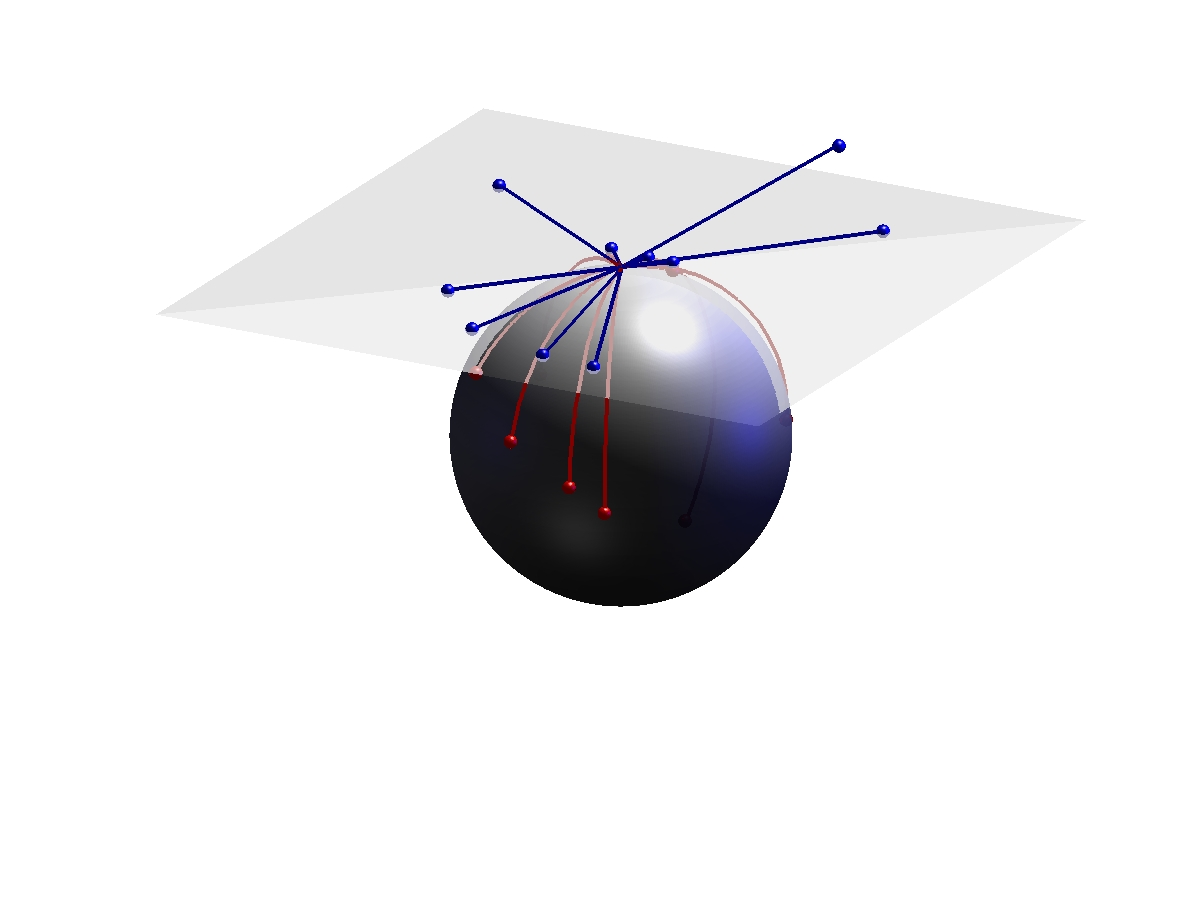
\includegraphics[width=1.2\textwidth]{spheres}
\end{center}
%\end{columns}
\end{frame}

%\begin{frame}
%\frametitle{D'Arcy Thompson's Generative Model}
%\begin{quote}
%``...diverse and dissimilar fishes can be referred as a whole to identical functions of very different co-ordinate systems...''
%\end{quote}
%\begin{center}
%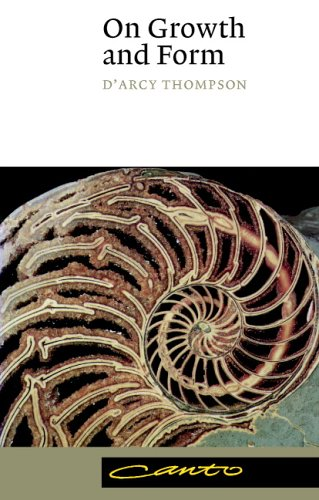
\includegraphics[height=0.4\textheight]{OGAF}
%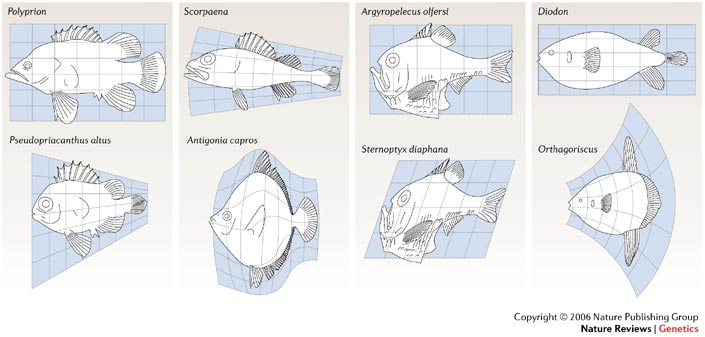
\includegraphics[height=0.4\textheight]{fish}
%\end{center}
%We can compute relative shapes using image registration.
%\end{frame}


    \subsection{Non-linear distances (manifolds)}
        \subsubsection{Manifolds}                \include{Manifolds}

    \subsection{Image registration for measuring distances}
    \subsection{Tangent space representations}
    \subsection{Scalar momenta}
    \subsection{Empirical examples}
        \subsubsection{Data}                     \begin{frame}
\frametitle{Real data}
\begin{columns}[c]
\column{0.5\textwidth}
Used 550 T1w brain MRI from IXI ({\bf I}nformation e{\bf X}traction from {\bf I}mages) dataset.

\url{http://www.brain-development.org/}

Data from three different hospitals in London:
\begin{itemize}
\item{Hammersmith Hospital using a Philips 3T system}
\item{Guy's Hospital using a Philips 1.5T system}
\item{Institute of Psychiatry using a GE 1.5T system}
\end{itemize}

\column{0.5\textwidth}
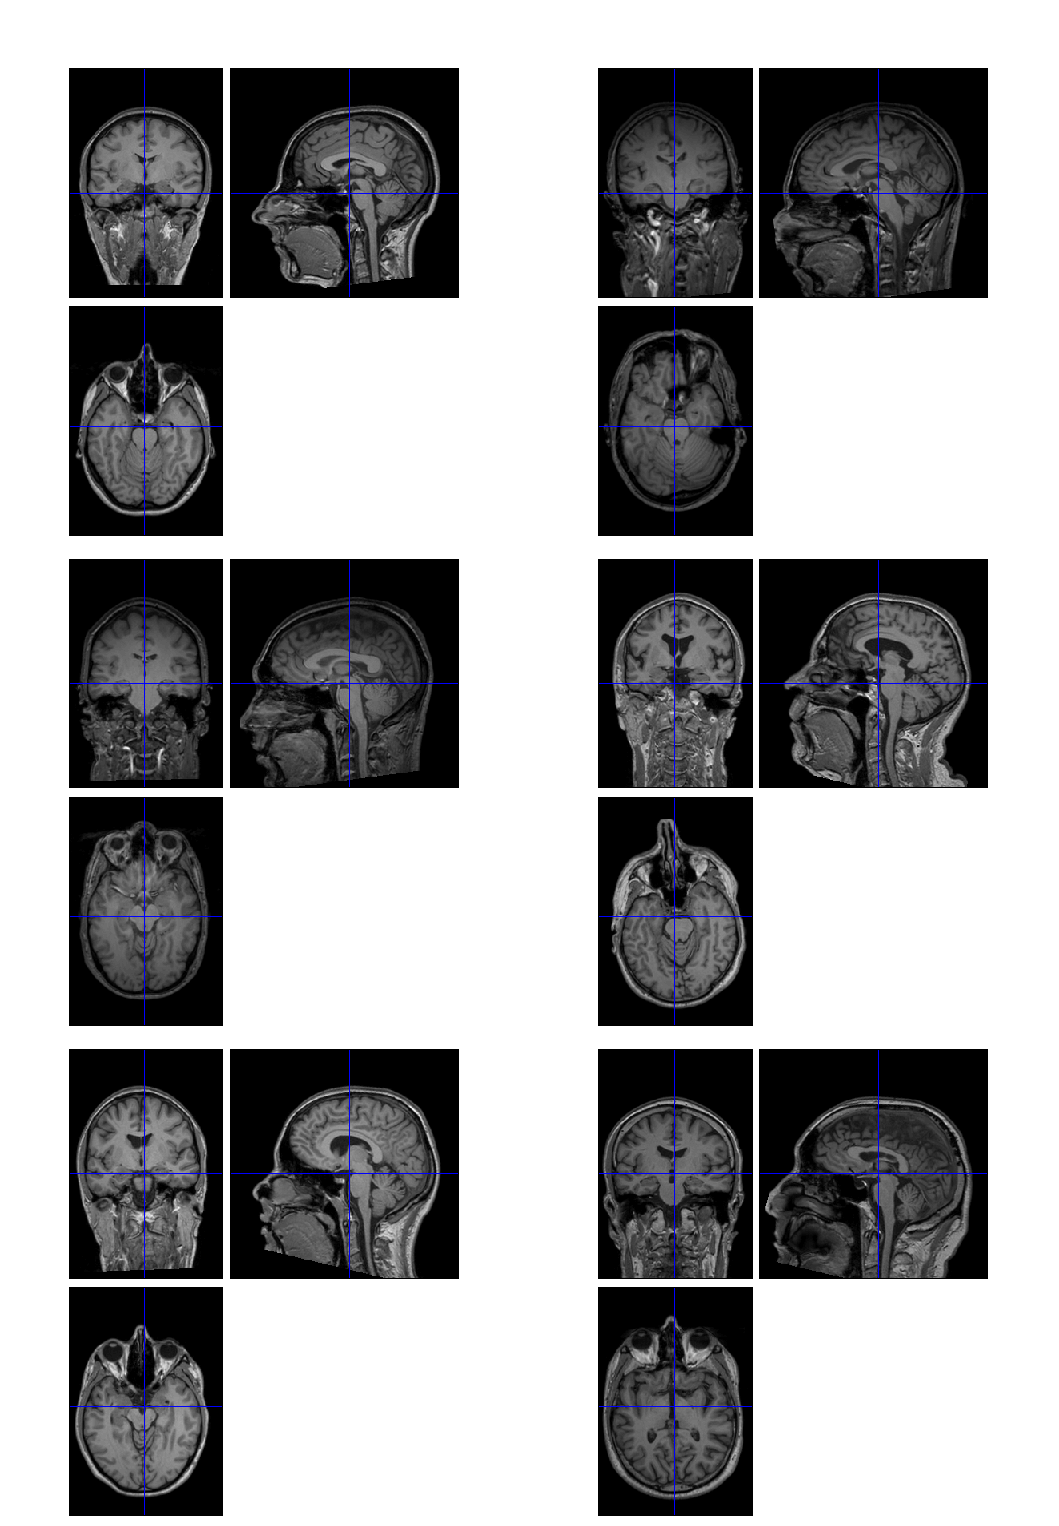
\includegraphics[width=0.9\textwidth]{orig_ixi}
\end{columns}
\end{frame}

\begin{frame}
\frametitle{Grey and White Matter}
\begin{columns}[c]
\column{0.26\textwidth}
Segmented into GM and WM.

Approximately aligned via rigid-body.
\column{0.75\textwidth}
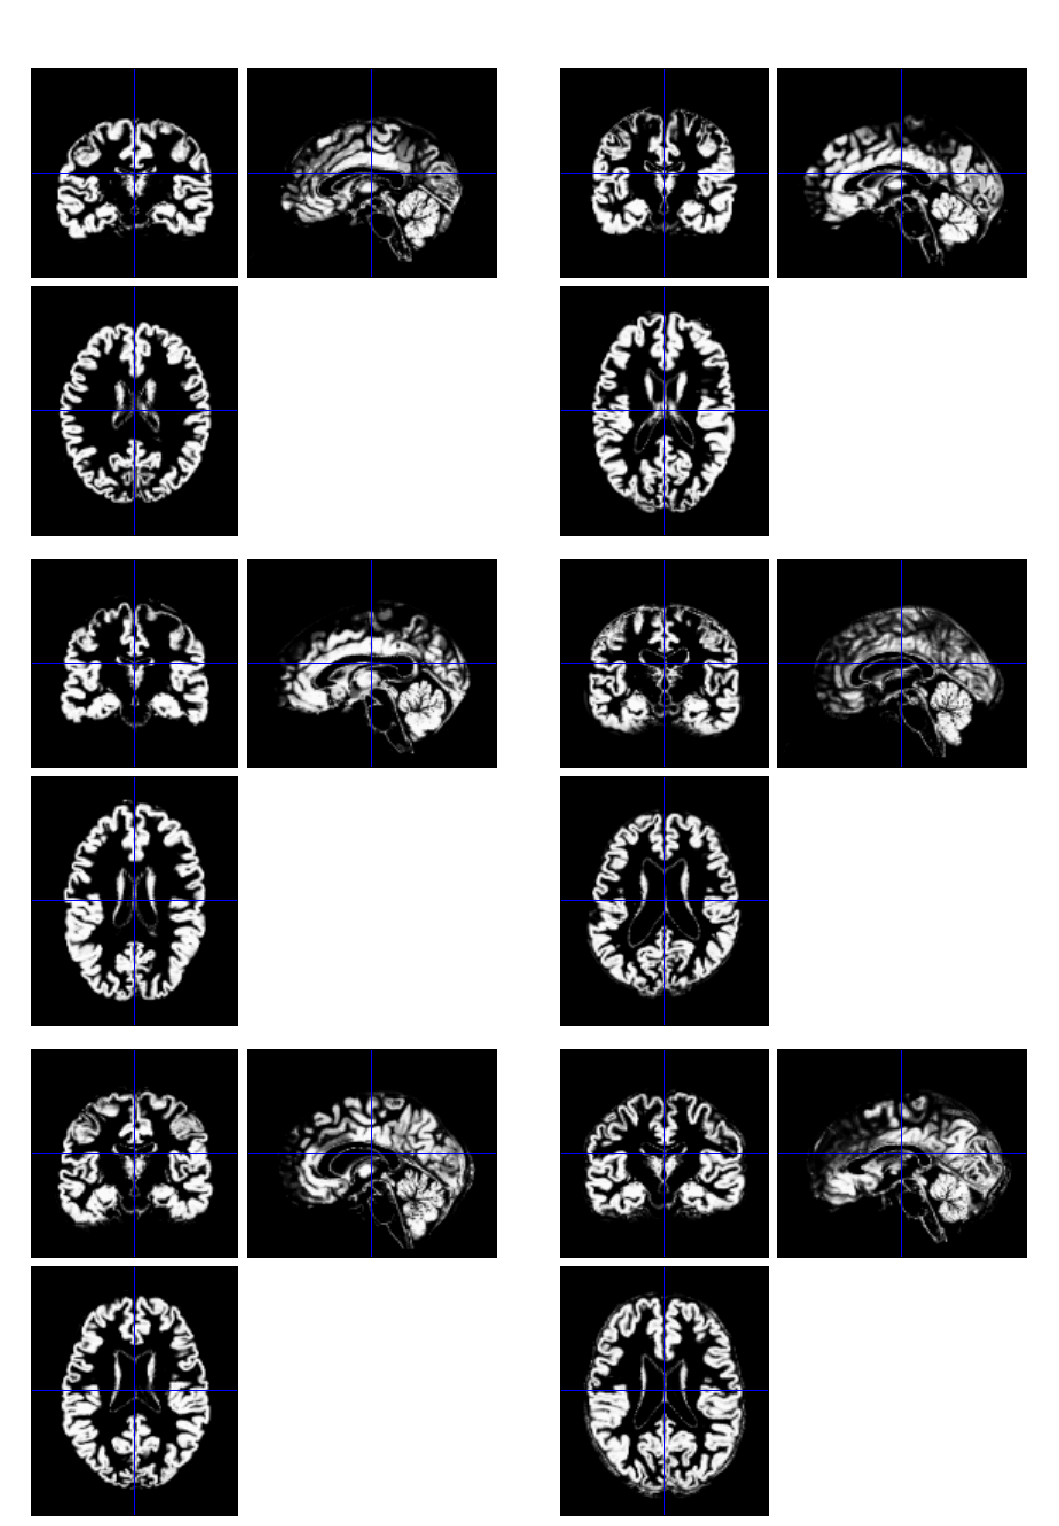
\includegraphics[width=0.5\textwidth]{gm_ixi}
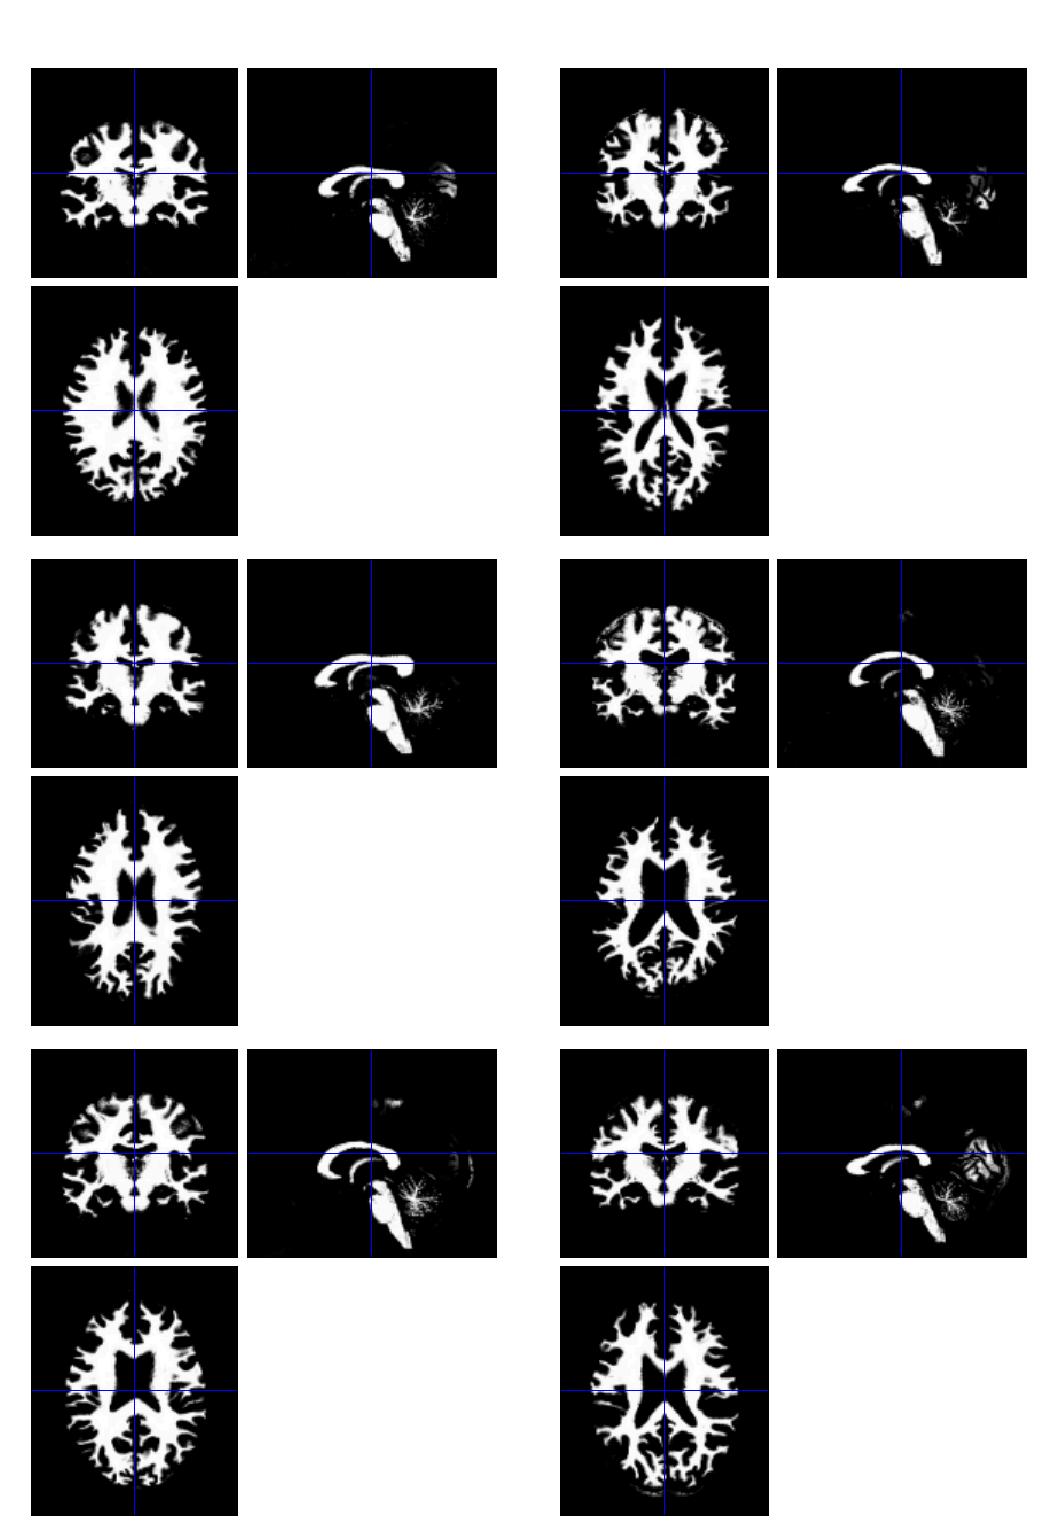
\includegraphics[width=0.5\textwidth]{wm_ixi}
\end{columns}

\begin{tiny}
Ashburner, J \& Friston, KJ. \emph{Unified segmentation}. NeuroImage 26(3):839--851 (2005).

\end{tiny}
\end{frame}

\begin{frame}
\frametitle{Diffeomorphic Alignment}
All GM and WM were diffeomorphically aligned to their common average-shaped template.
\begin{center}
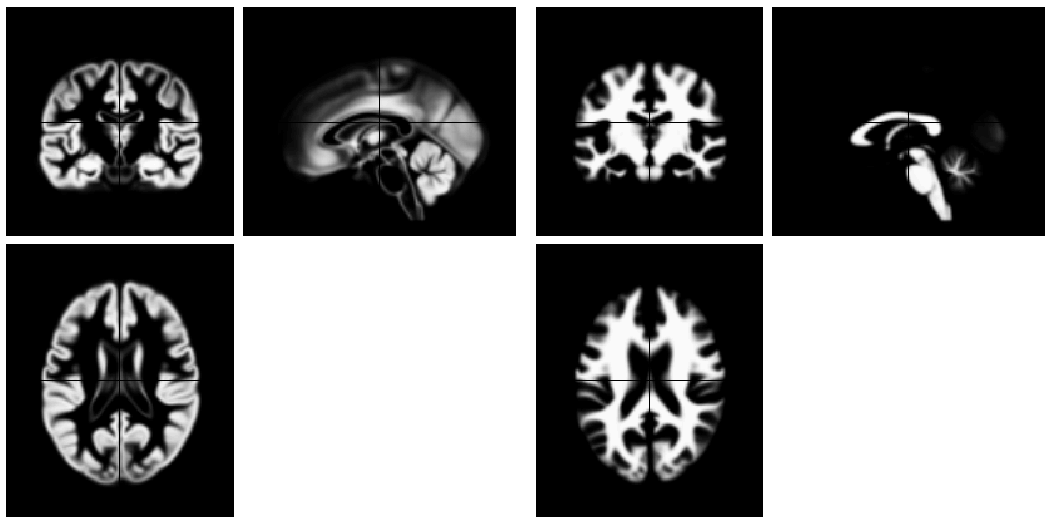
\includegraphics[width=.8\textwidth]{template}
\end{center}

\begin{tiny}
Ashburner, J \& Friston, KJ. \emph{Diffeomorphic registration using geodesic shooting and Gauss-Newton optimisation}. NeuroImage 55(3):954--967 (2011).

Ashburner, J \& Friston, KJ. \emph{Computing average shaped tissue probability templates}. NeuroImage 45(2):333--341 (2009).

\end{tiny}
\end{frame}


        \subsubsection{Features}                 \begin{frame}
\frametitle{Volumetric Features}
\begin{columns}[c]
\column{0.33\textwidth}
A number of features were used for pattern recognition.

Firstly, two features relating to relative volumes.

Initial velocity divergence is similar to logarithms of Jacobian determinants.
\column{0.33\textwidth}
Jacobian Determinants

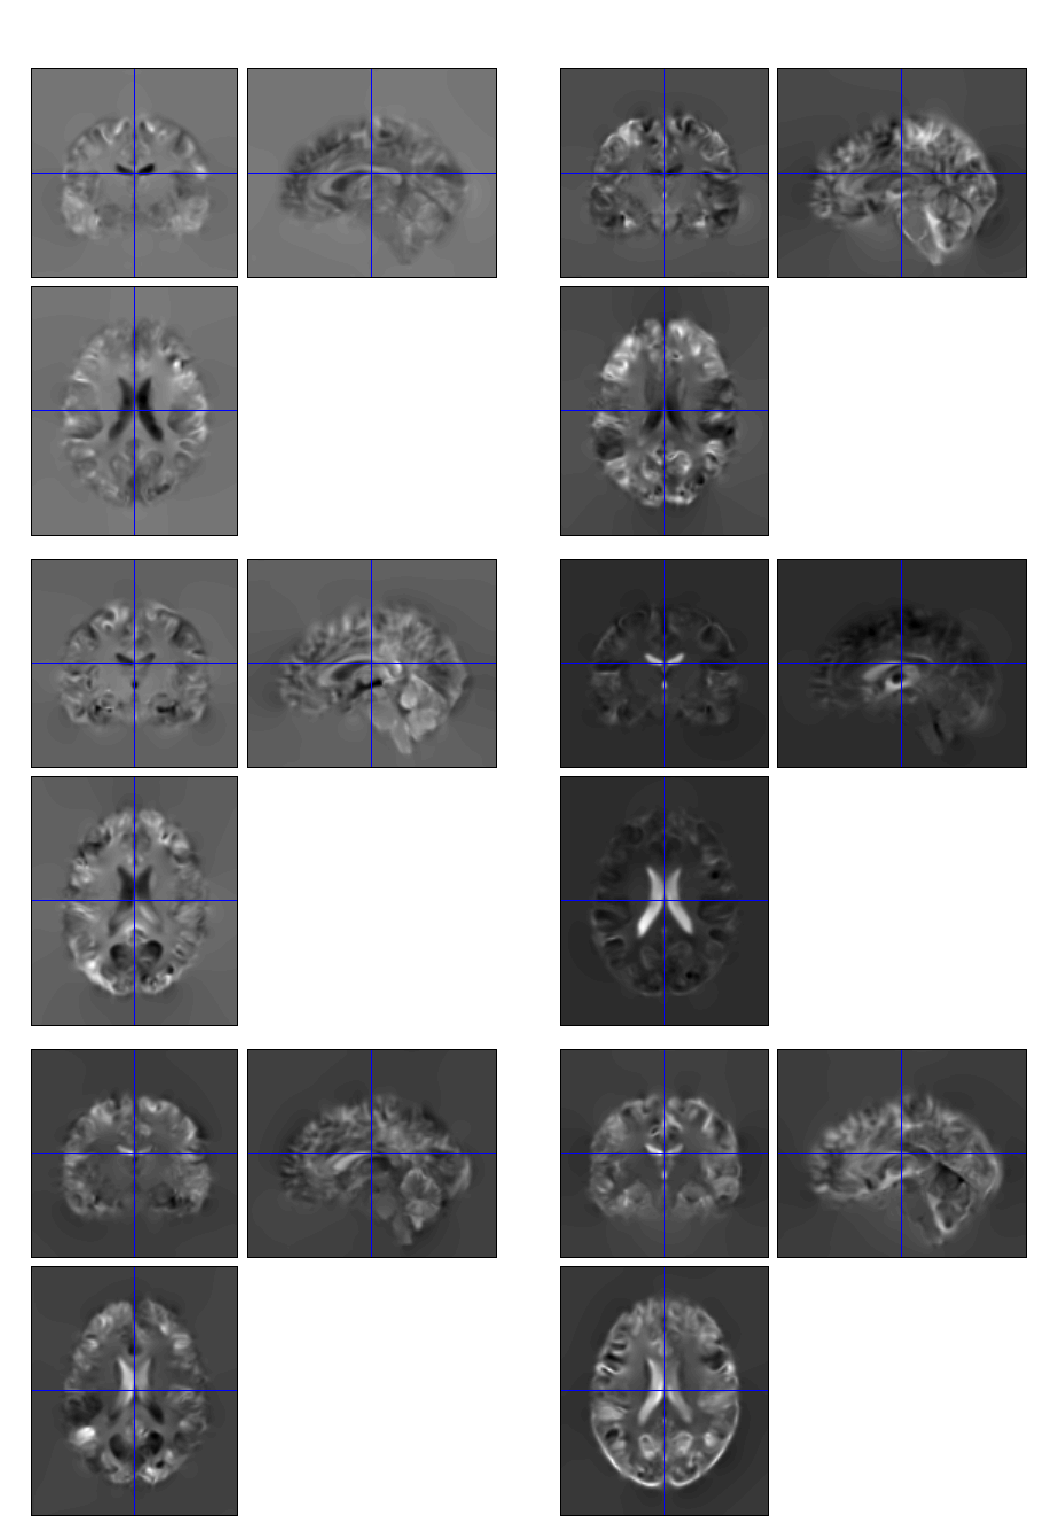
\includegraphics[width=1\textwidth]{jac_ixi}
\column{0.33\textwidth}
Initial Velocity Divergence
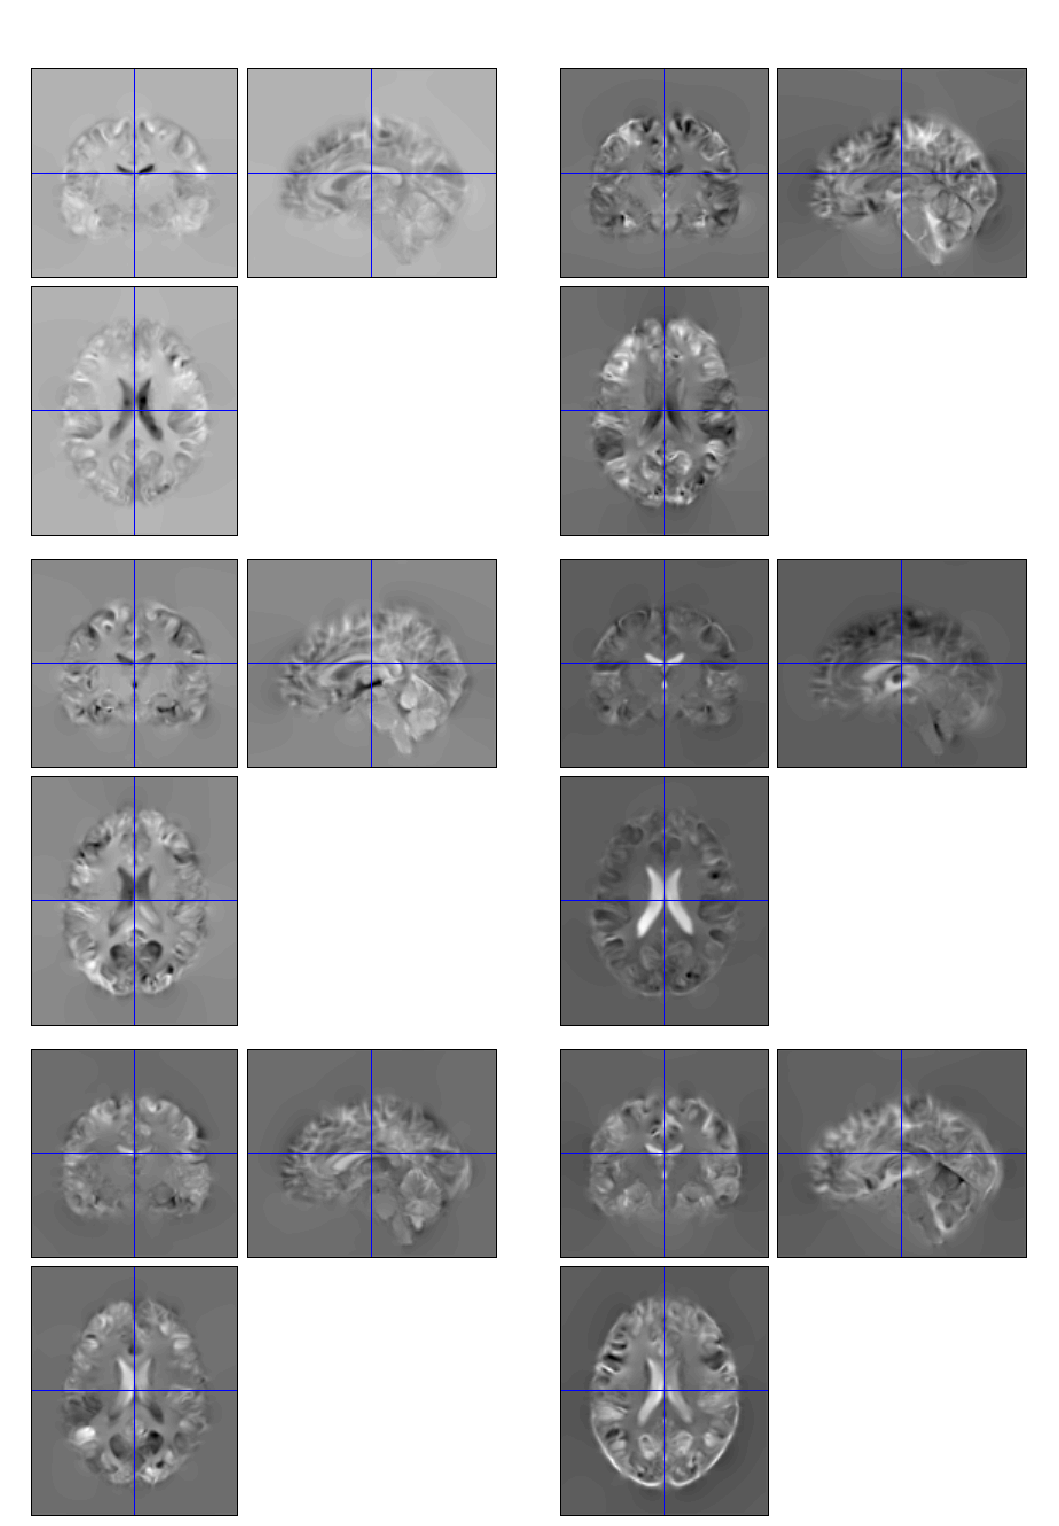
\includegraphics[width=1\textwidth]{div_ixi}
\end{columns}
\end{frame}

%%%%%%%%%%%%%%%%%%%%%%%%%%%%%%%%%%%%%%%%%%%%%%%%%%%%%%%%%%%%%%%
\begin{frame}
\frametitle{Grey Matter Features}
\begin{columns}[c]
\column{0.33\textwidth}
Rigidly Registered GM

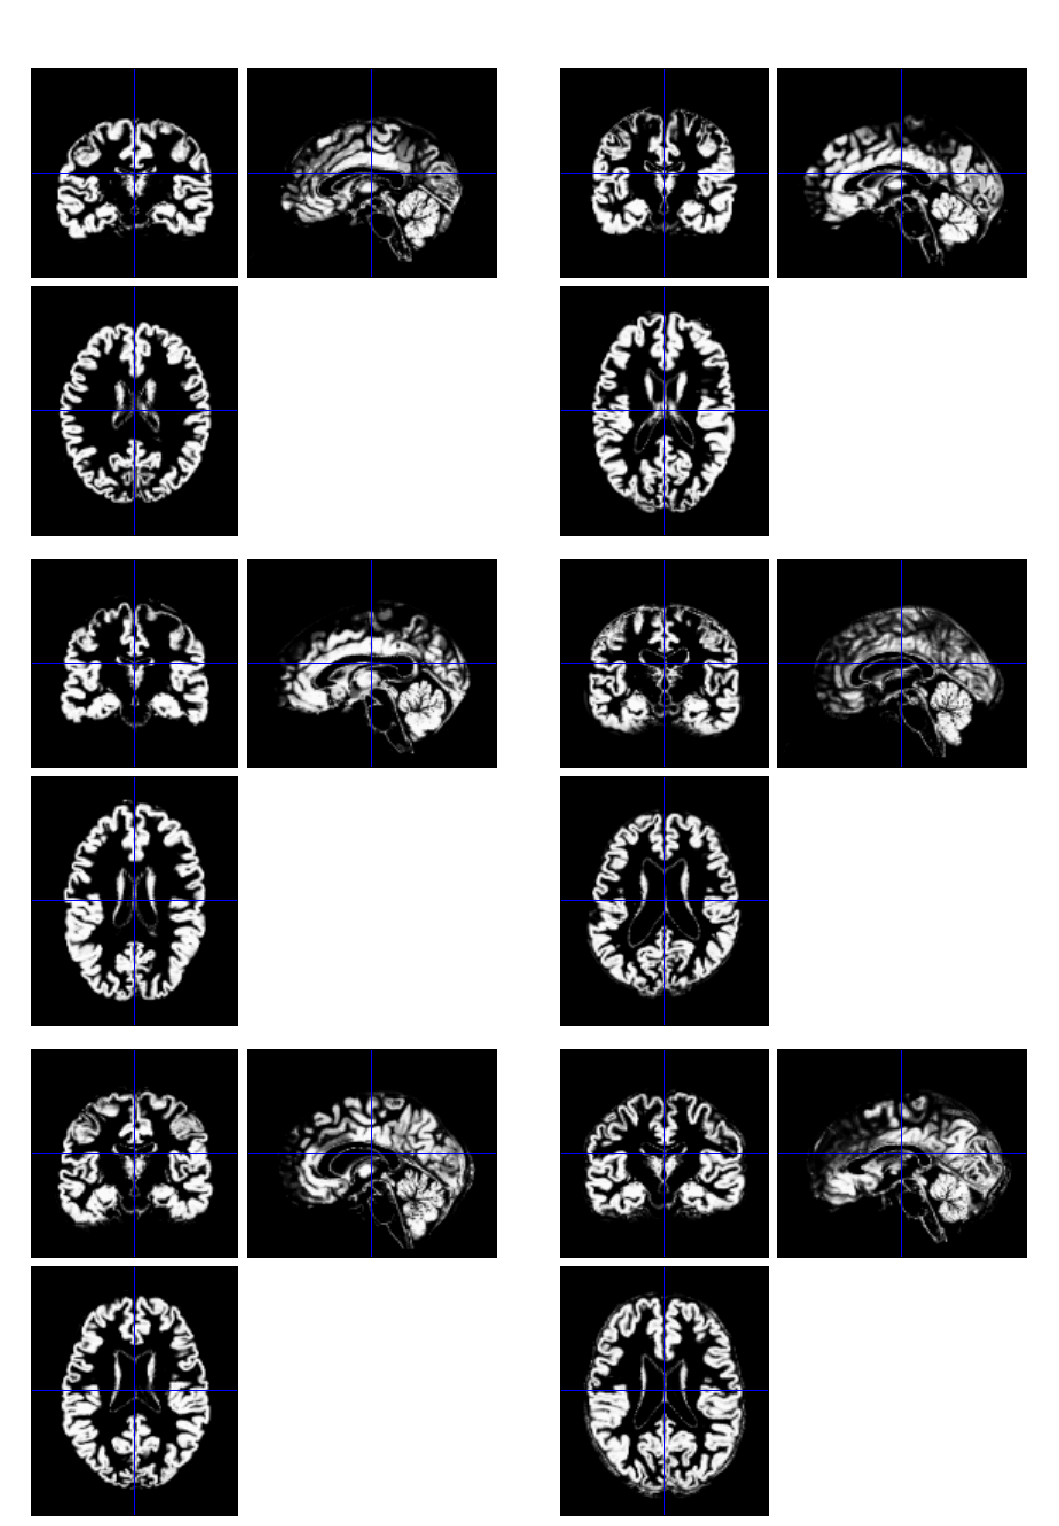
\includegraphics[width=1\textwidth]{gm_ixi}

\column{0.33\textwidth}
Nonlinearly Registered GM

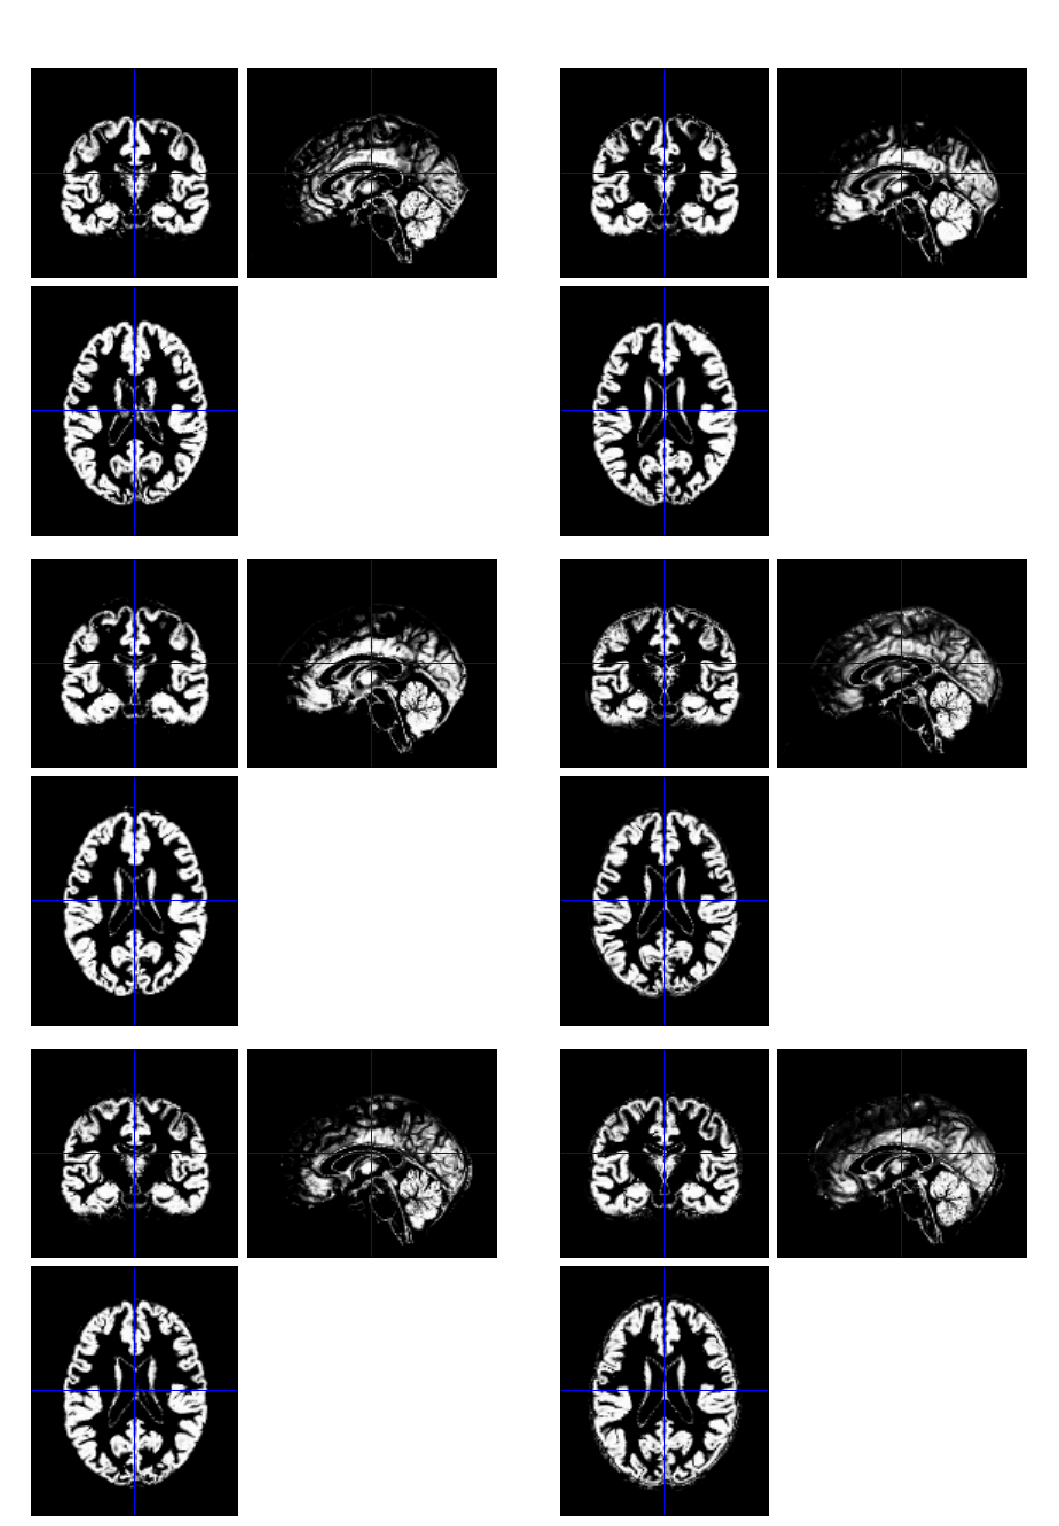
\includegraphics[width=1\textwidth]{wc1_ixi}
\column{0.33\textwidth}
Registered and Jacobian Scaled GM

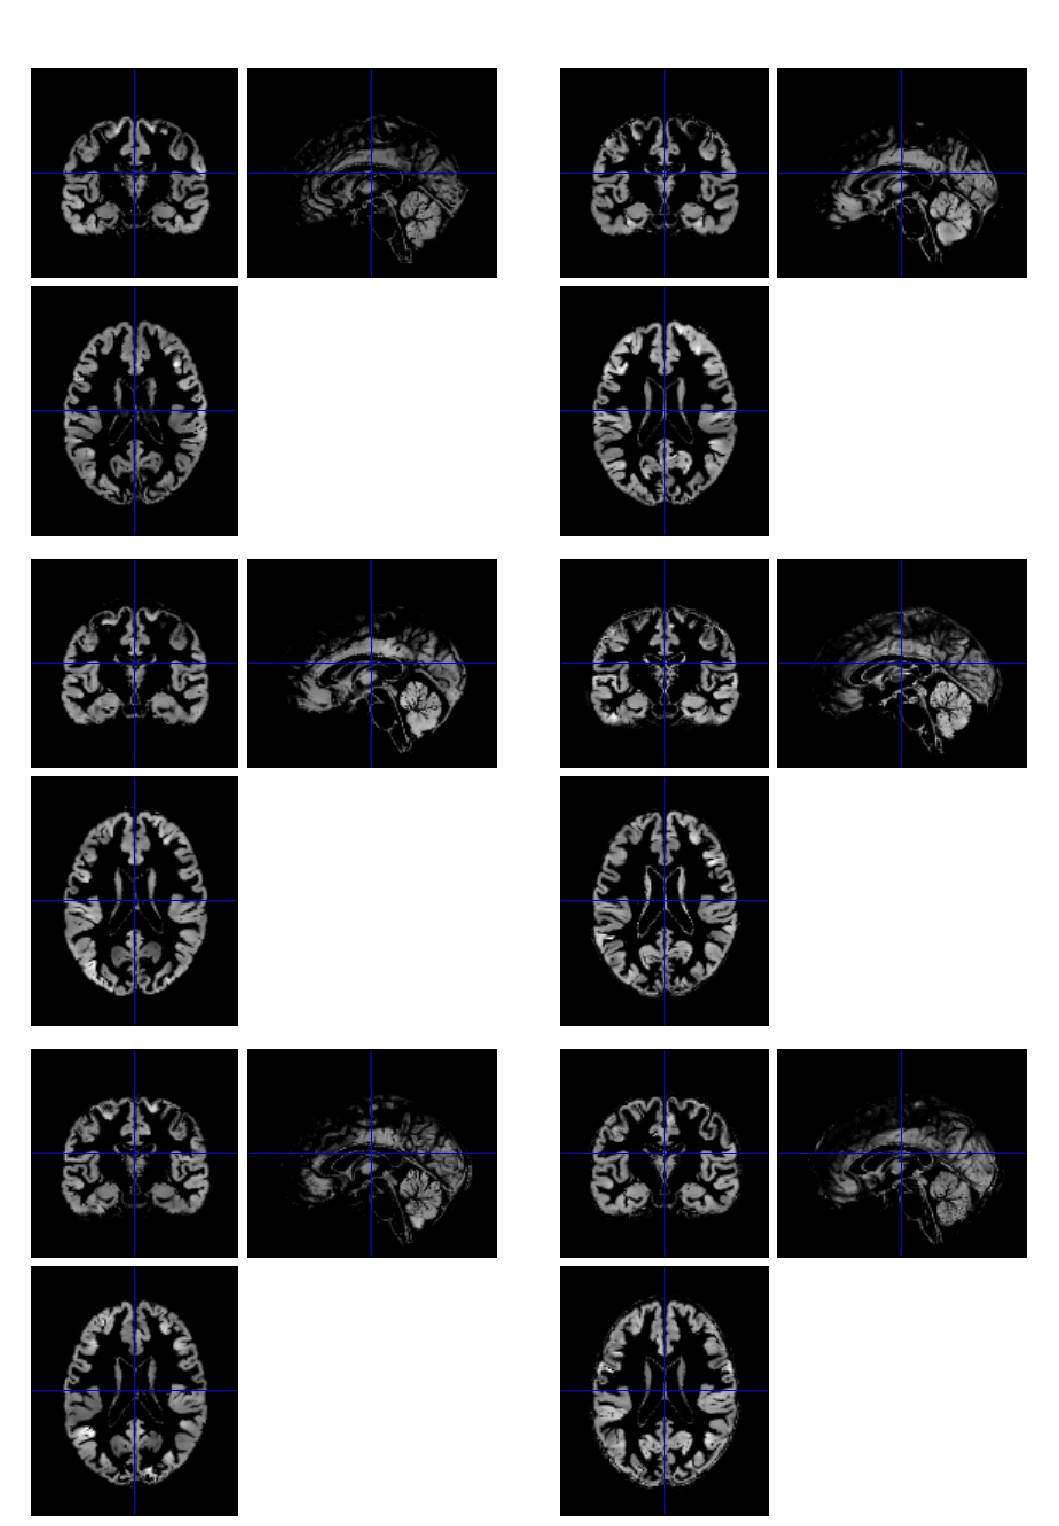
\includegraphics[width=1\textwidth]{mwc1_ixi}
\end{columns}
\end{frame}

%%%%%%%%%%%%%%%%%%%%%%%%%%%%%%%%%%%%%%%%%%%%%%%%%%%%%%%%%%%%%%%
%%%%%%%%%%%%%%%%%%%%%%%%%%%%%%%%%%%%%%%%%%%%%%%%%%%%%%%%%%%%%%%
\begin{frame}
\frametitle{``Scalar Momentum'' Features}
\begin{columns}[c]
\column{0.33\textwidth}
``Scalar momentum'' actually has two components because GM was matched with GM and WM was matched with WM.
\column{0.33\textwidth}
First Momentum Component

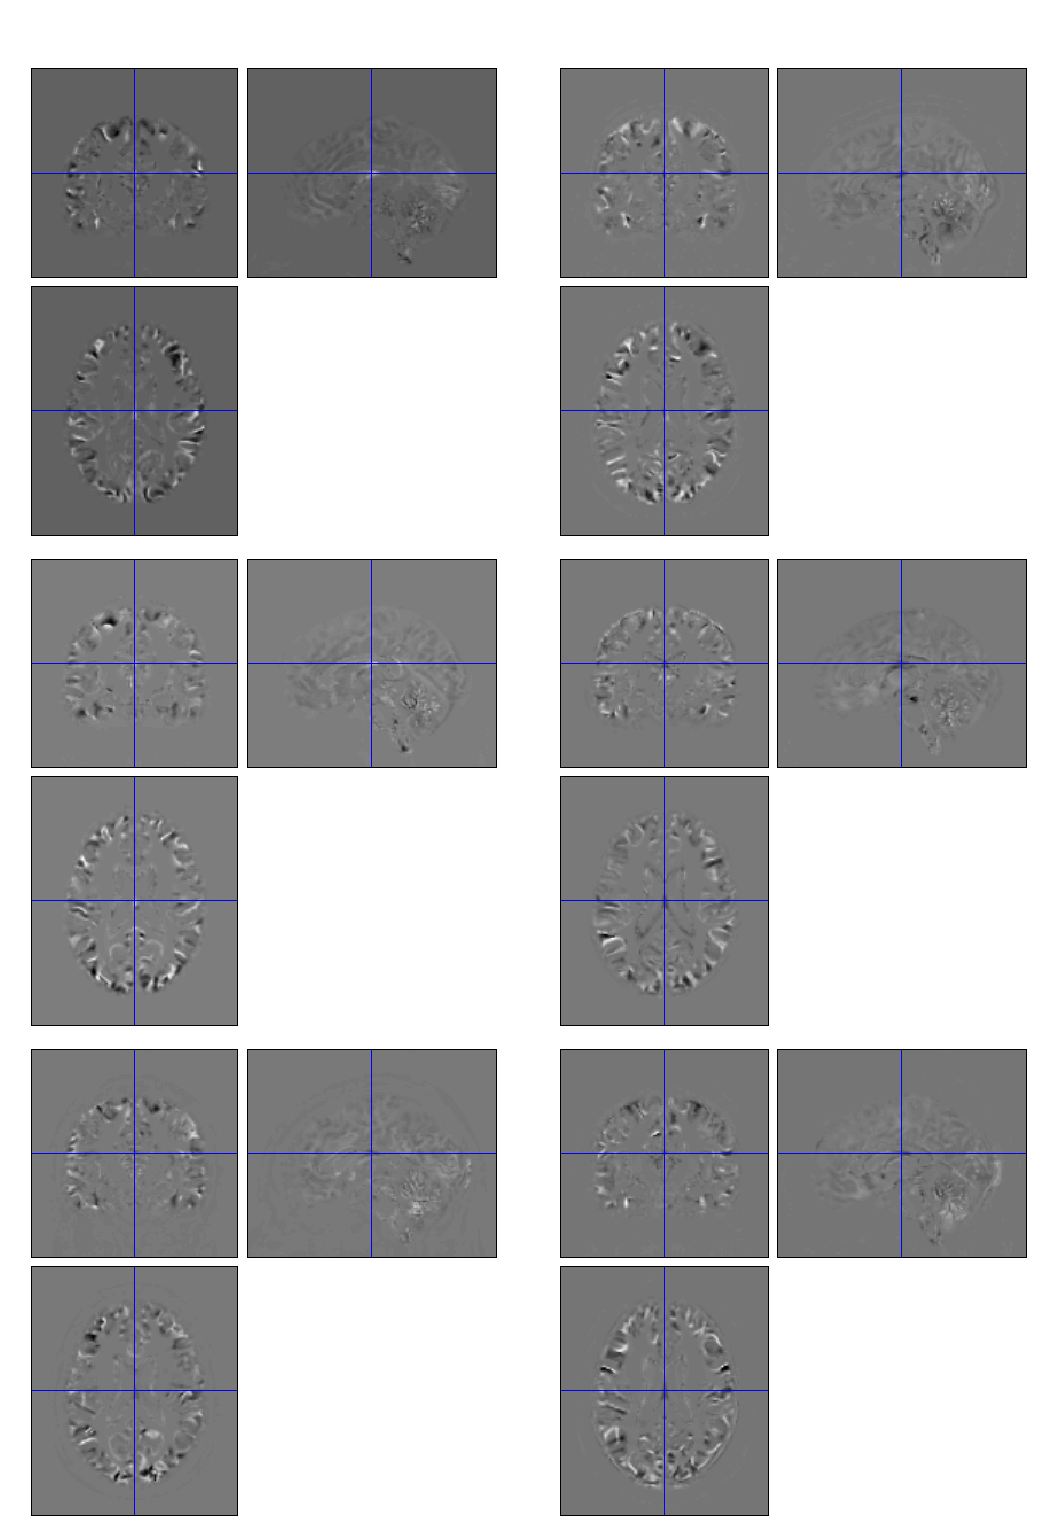
\includegraphics[width=1\textwidth]{resids1_ixi}
\column{0.33\textwidth}
Second Momentum Component

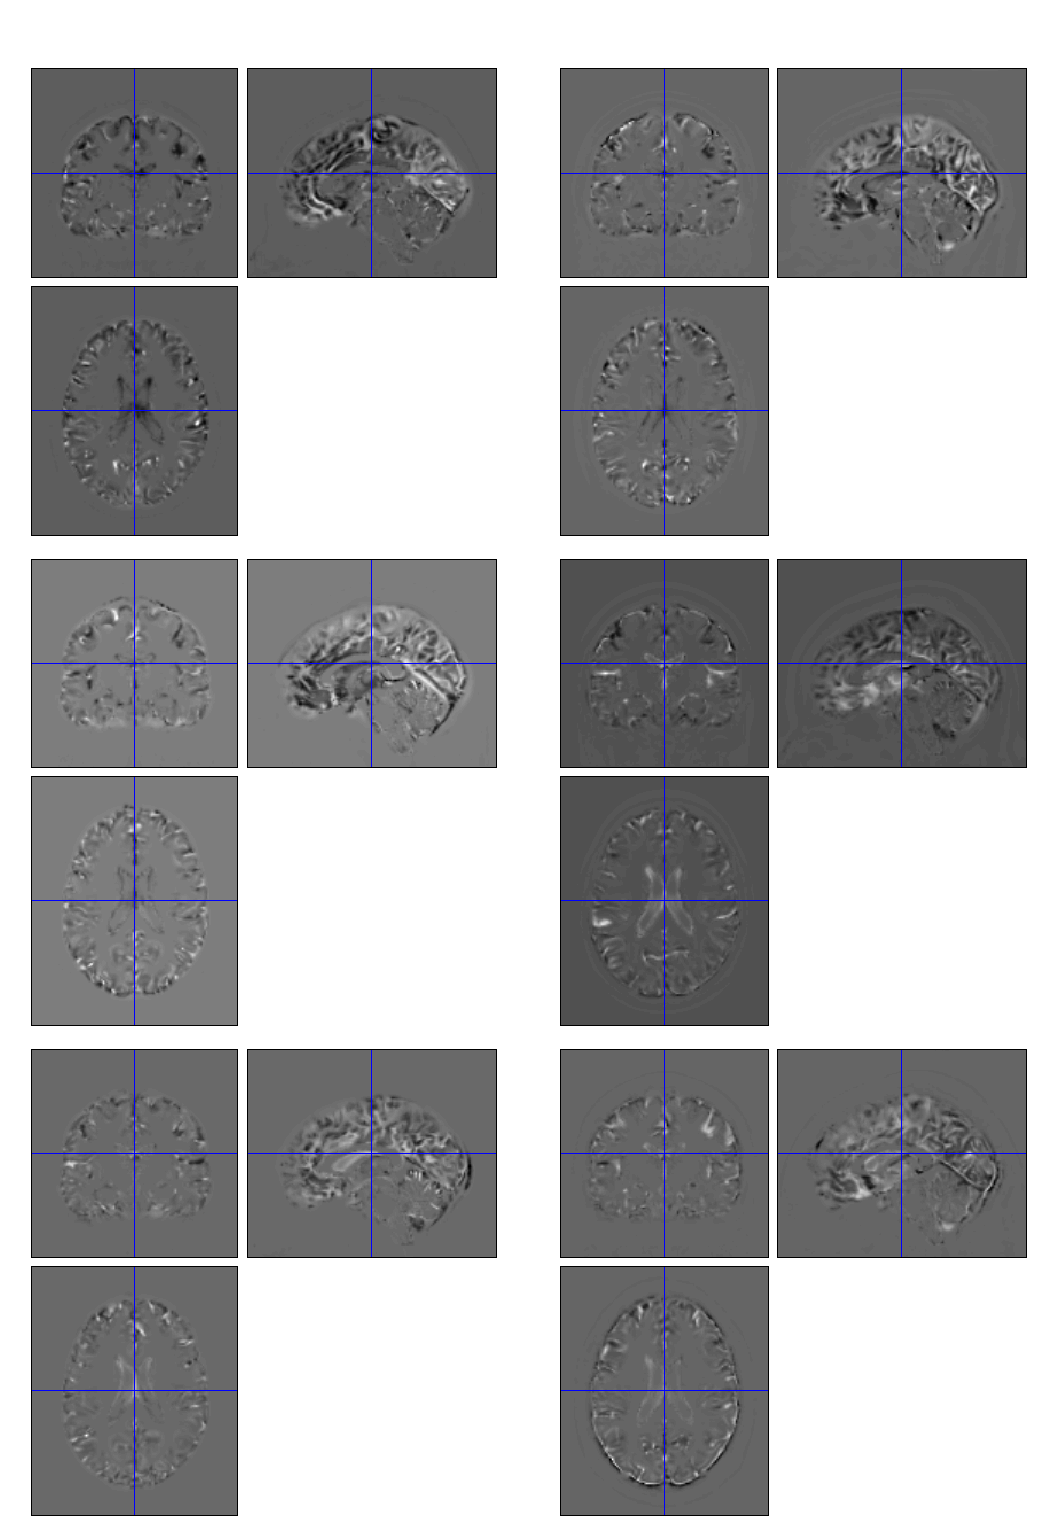
\includegraphics[width=1\textwidth]{resids2_ixi}
\end{columns}
\end{frame}



        \subsubsection{Results}                  \begin{frame}
\frametitle{Age Regression}
Linear Gaussian Process Regression to predict subject ages.
\begin{columns}[c]
\column{0.5\textwidth}
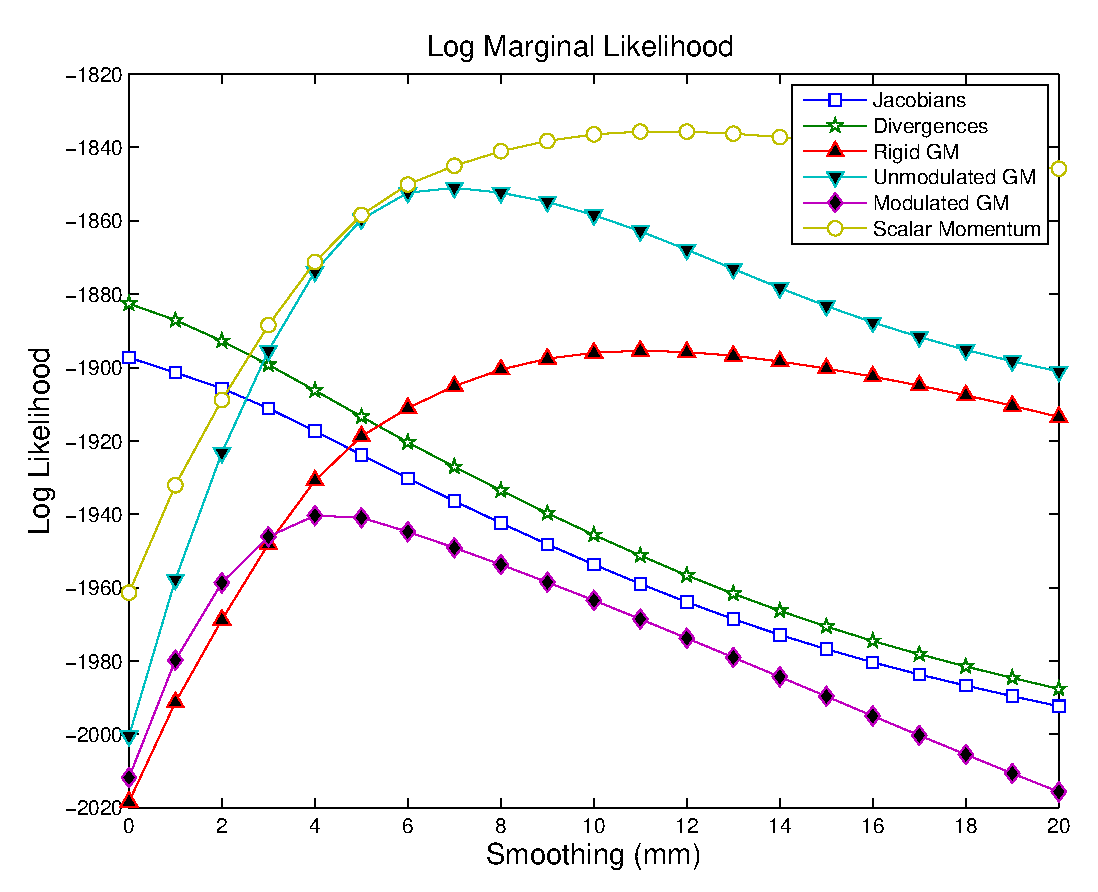
\includegraphics[width=1\textwidth]{age_loglikelihood}
\column{0.5\textwidth}
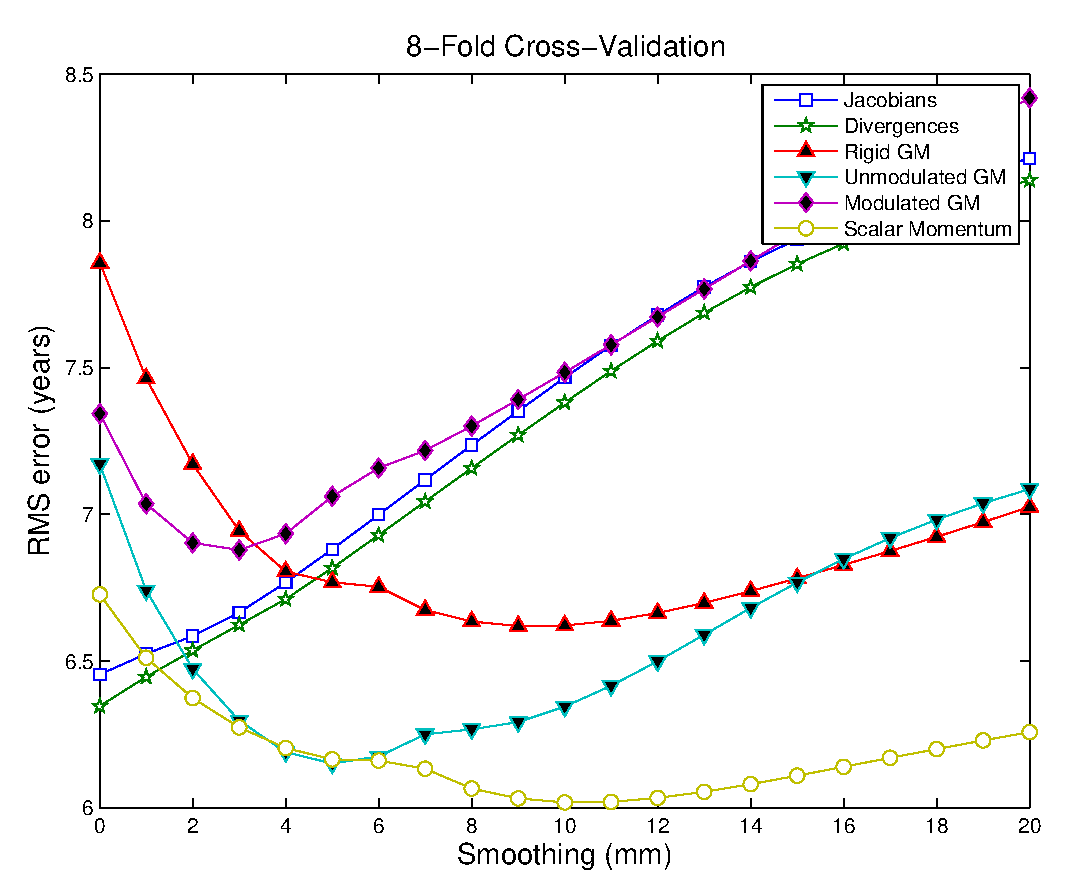
\includegraphics[width=1\textwidth]{age_rms}
\end{columns}

\begin{tiny}
Rasmussen, CE \& Williams, CKI. \emph{Gaussian processes for machine learning}. Springer (2006).

\end{tiny}
\end{frame}

%%%%%%%%%%%%%%%%%%%%%%%%%%%%%%%%%%%%%%%%%%%%%%%%%%%%%%%%%%%%%%%
\begin{frame}
\frametitle{Sex Classification}
Linear Gaussian Process Classification (EP) to predict sexes.
\begin{columns}[c]
\column{0.5\textwidth}
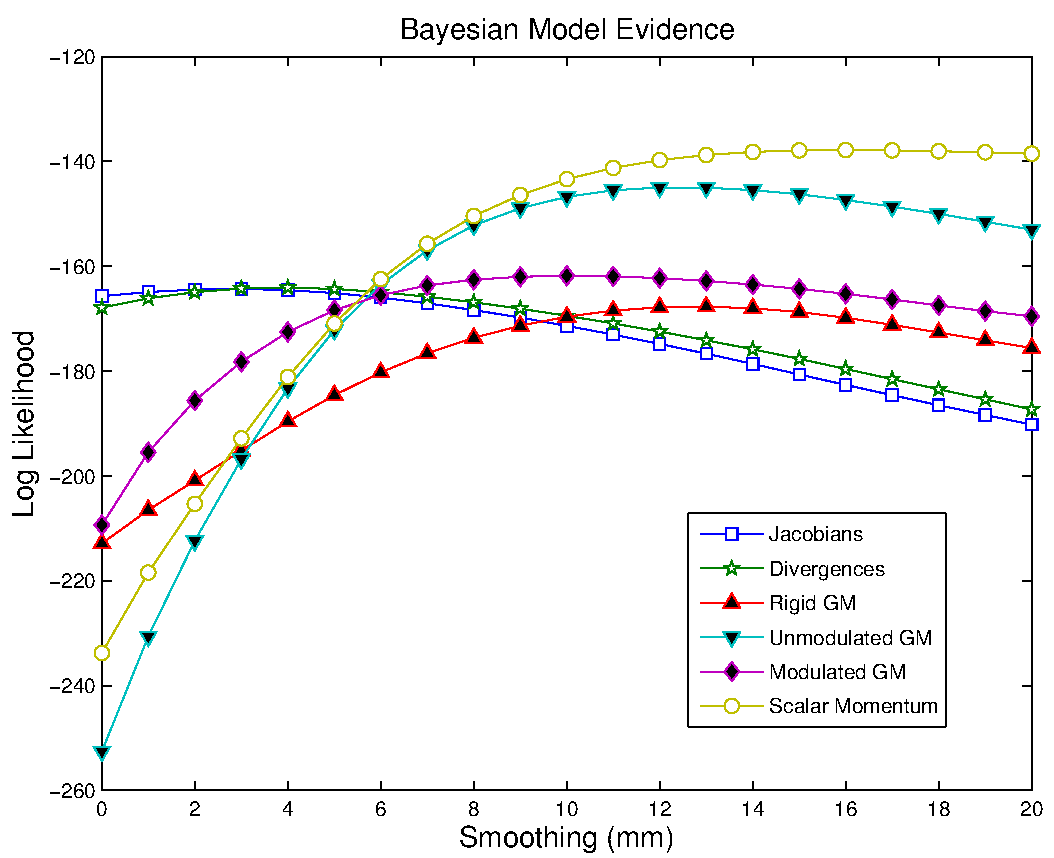
\includegraphics[width=1\textwidth]{sex_loglikelihood}
\column{0.5\textwidth}
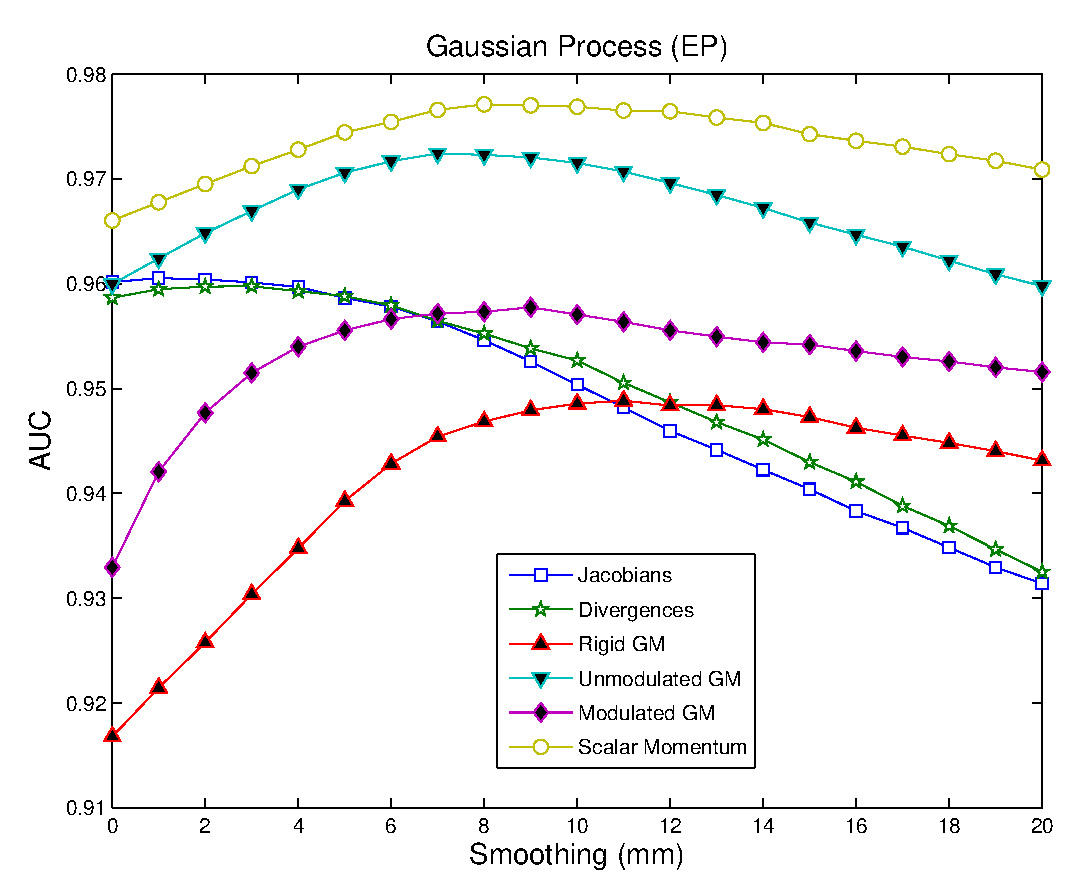
\includegraphics[width=1\textwidth]{sex_auc_GP}
\end{columns}

\begin{tiny}
Rasmussen, CE \& Williams, CKI. \emph{Gaussian processes for machine learning}. Springer (2006).

\end{tiny}
\end{frame}

%%%%%%%%%%%%%%%%%%%%%%%%%%%%%%%%%%%%%%%%%%%%%%%%%%%%%%%%%%%%%%%
%\begin{frame}
%\frametitle{Sex Classification}
%Linear SVM versus Gaussian Process Classification (EP).
%\begin{columns}[c]
%\column{0.5\textwidth}
%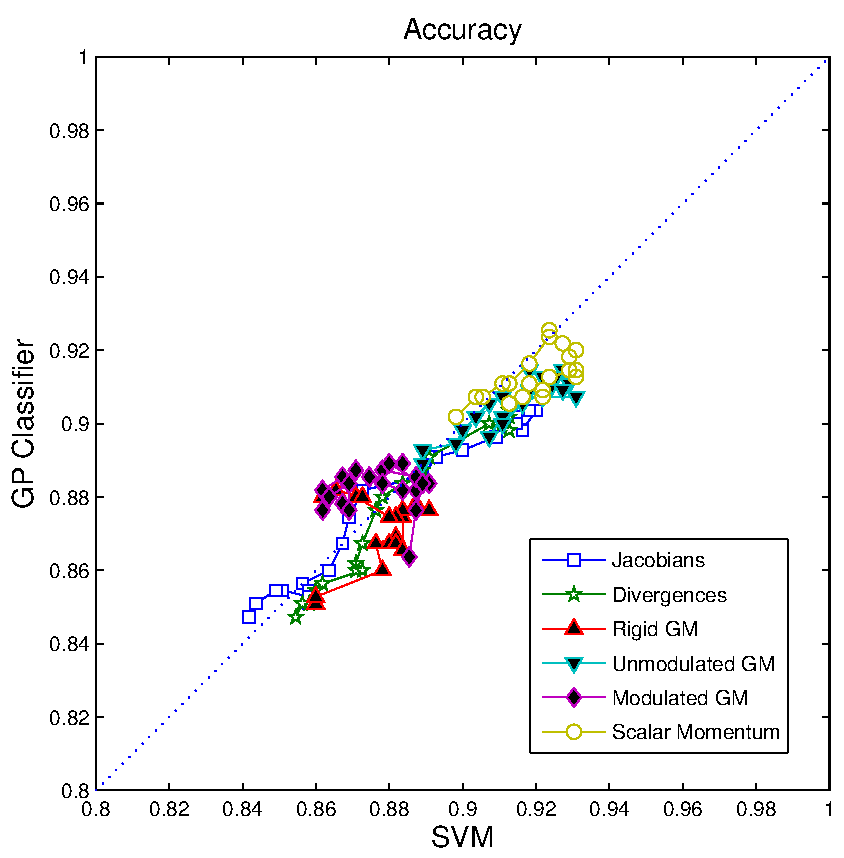
\includegraphics[width=1\textwidth]{sex_SVM_v_GP_acc}
%\column{0.5\textwidth}
%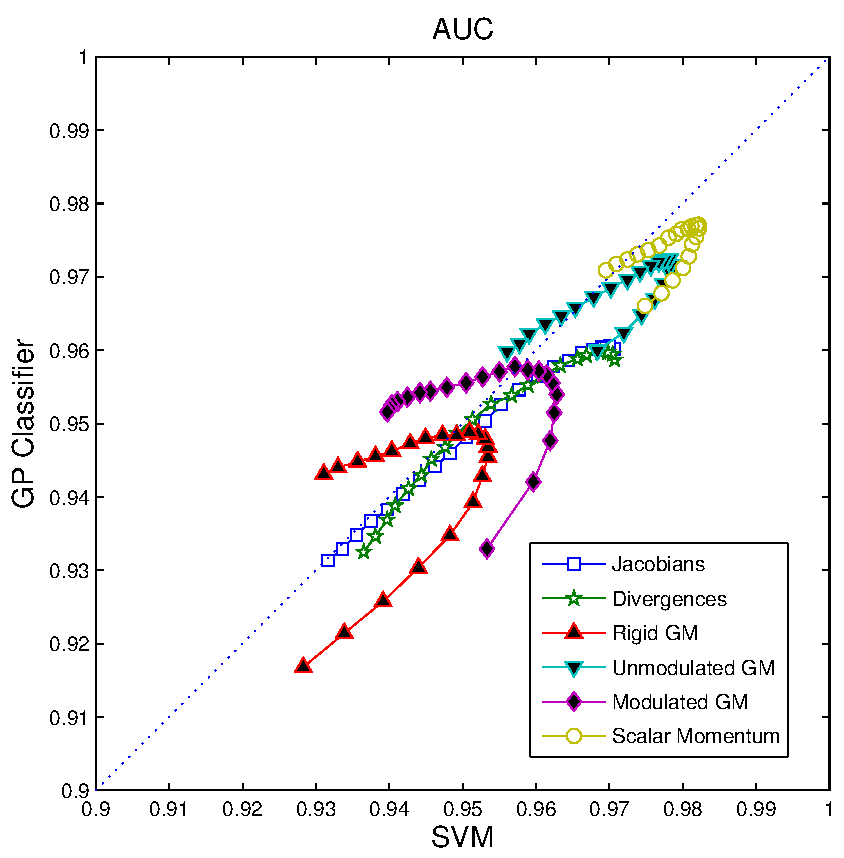
\includegraphics[width=1\textwidth]{sex_SVM_v_GP_AUC}
%\end{columns}
%\end{frame}

%%%%%%%%%%%%%%%%%%%%%%%%%%%%%%%%%%%%%%%%%%%%%%%%%%%%%%%%%%%%%%%

\begin{frame}
\frametitle{Predictive Accuracies}
\begin{columns}[c]
\column{0.5\textwidth}

Age

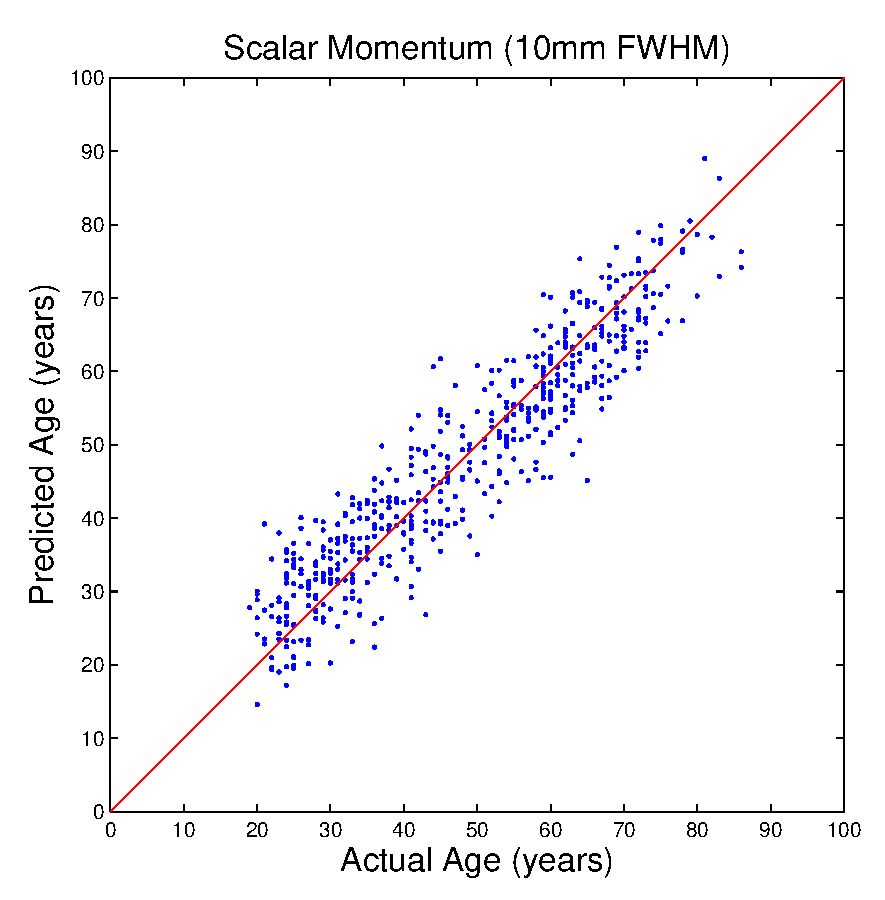
\includegraphics[width=1\textwidth]{age_predictions}
\column{0.5\textwidth}

Sex

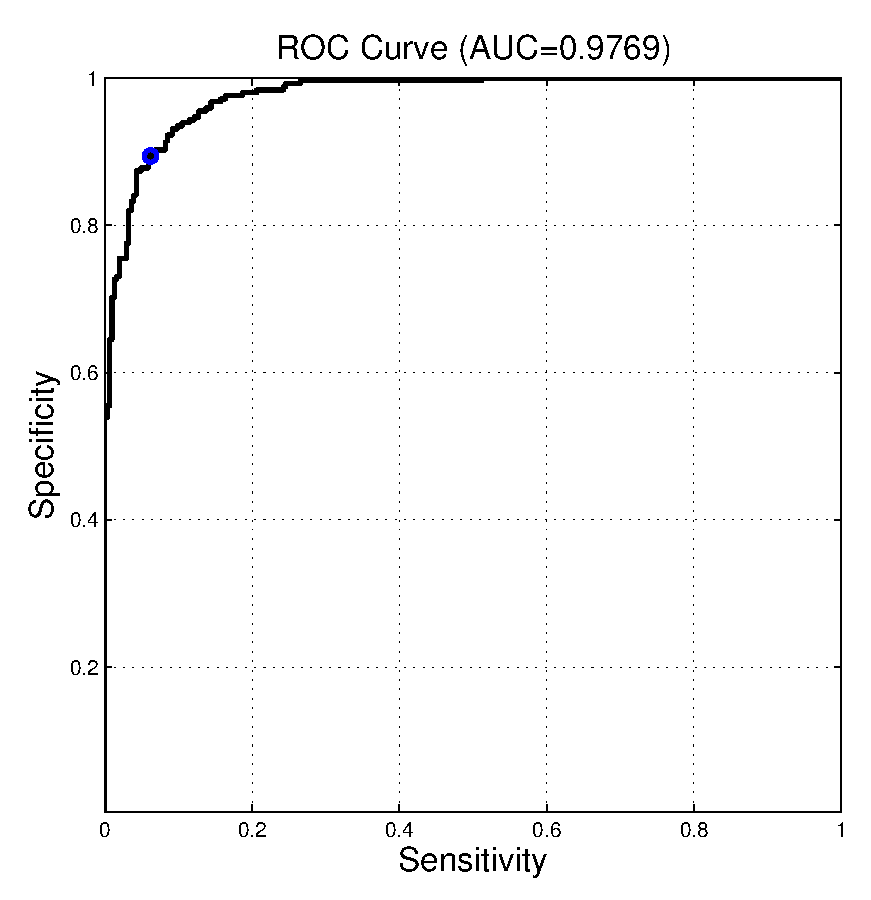
\includegraphics[width=1\textwidth]{sex_roc}
\end{columns}
\end{frame}

\begin{frame}
\frametitle{Conclusions}
\begin{itemize}
\item{Scalar momentum (with about 10mm smoothing) appears to be a useful feature set.}
\item{Jacobian-scaled warped GM is surprisingly poor.}
%\item{SVC slightly more accurate than GP (but we knew that already).}
\item{Amount of spatial smoothing makes a big difference.}
\item{Further dependencies on the details of the registration still need exploring.}
\end{itemize}
\end{frame}
%%%%%%%%%%%%%%%%%%%%%%%%%%%%%%%%%%%%%%%%%%%%%%%%%%%%%%%%%%%%%%%
%\begin{frame}
%\frametitle{Additional references}
%\begin{itemize}
%\item{Ashburner, J \& Kl\"oppel, K. \emph{Multivariate models of inter-subject anatomical variability}. NeuroImage 56(2):422--439 (2011).}
%\item{Ashburner, J \& Friston, KJ. \emph{Diffeomorphic registration using geodesic shooting and Gauss-Newton optimisation}. NeuroImage 55(3):954--967 (2011).}
%\end{itemize}
%\end{frame}

\begin{frame}
\begin{center}
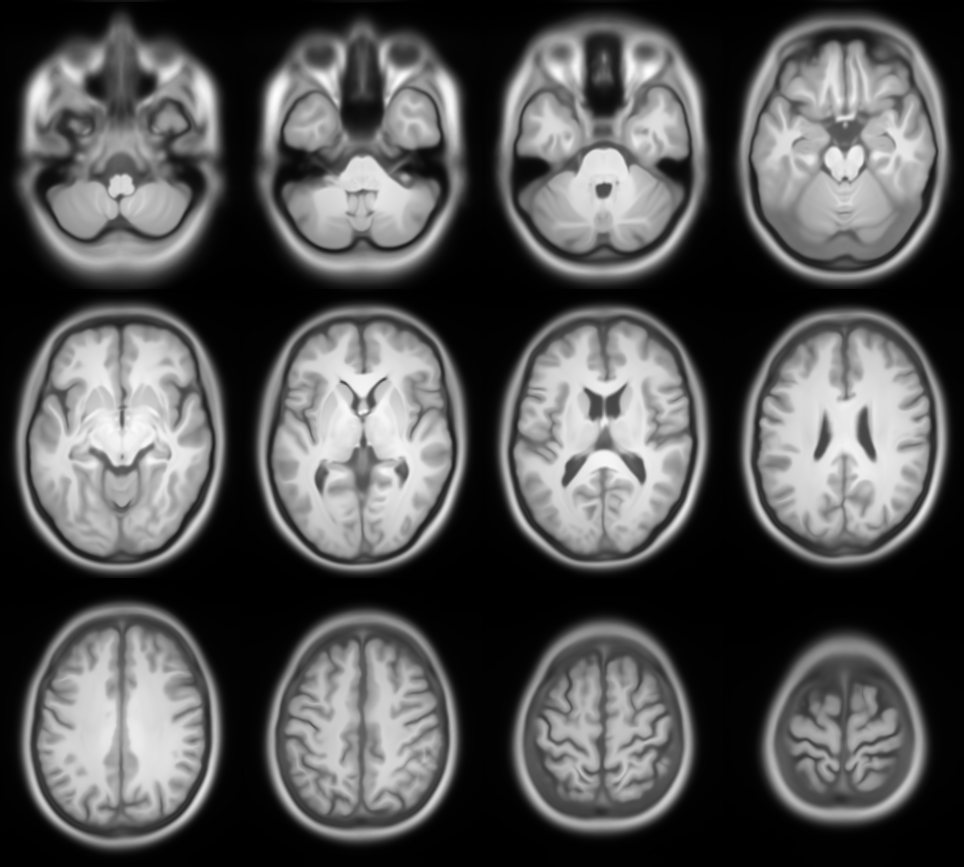
\includegraphics[width=.8\textwidth]{hyper_male}
\end{center}
\end{frame}

\begin{frame}
\begin{center}
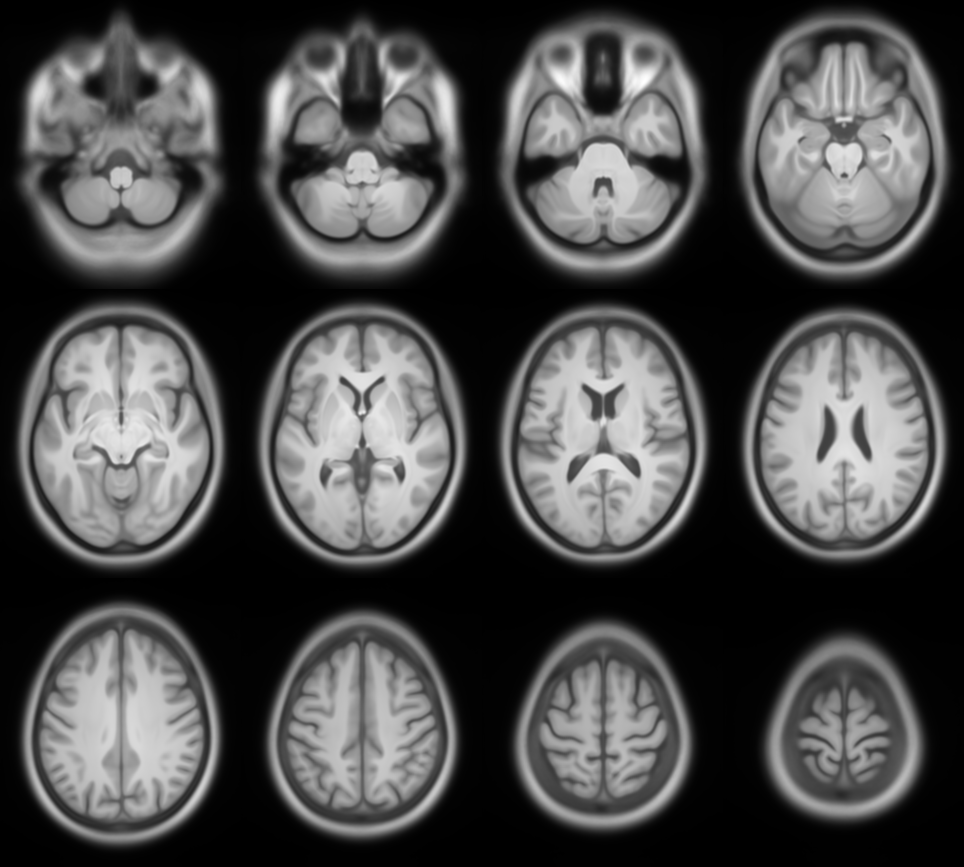
\includegraphics[width=.8\textwidth]{avgT1}
\end{center}
\end{frame}

\begin{frame}
\begin{center}
\includegraphics[width=.8\textwidth]{hyper_female}
\end{center}
\end{frame}




%    \subsection{Examples of features}     \begin{frame}
\frametitle{Example Images}
Some example (non-brain) images.
\begin{center}
\includegraphics[width=0.9\textwidth]{original}
\end{center}
\end{frame}

%\begin{frame}
%\frametitle{Samples from a Linear Generative Model}
%Did the images come from a model like this?
%\begin{center}
%\includegraphics[width=0.9\textwidth]{simulated_lin}
%\end{center}
%\end{frame}

%\begin{frame}
%\frametitle{Samples from a Geometric Generative Model}
%Or one like this?
%\begin{center}
%\includegraphics[width=0.9\textwidth]{simulated}
%\end{center}
%\end{frame}

\begin{frame}
\frametitle{Registered Images}
We could register the images to their average shape...
\begin{center}
\includegraphics[width=0.9\textwidth]{warped}
\end{center}
\end{frame}

\begin{frame}
\frametitle{Deformations}
...and study the deformations...
\begin{center}
\includegraphics[width=0.9\textwidth]{deformations}
\end{center}
\end{frame}

\begin{frame}
\frametitle{Jacobian Determinants}
...or the relative volumes...
\begin{center}
\includegraphics[width=0.9\textwidth]{jacobians}
\end{center}
\end{frame}

\begin{frame}
\frametitle{Scalar Momentum}
... or ``scalar momentum'' (Singh et al, MICCAI 2010).
\begin{center}
\includegraphics[width=0.9\textwidth]{alpha}
\end{center}
\end{frame}

\begin{frame}
\frametitle{Reconstructed Images}
Reconstructions from template and scalar momenta.
\begin{center}
\includegraphics[width=0.9\textwidth]{reconstructed}
\end{center}
\end{frame}

%\begin{frame}
%\frametitle{Evolution}
%\begin{center}
%\includegraphics[width=.8\textwidth]{evolution}\par
%\begin{tiny}
%Singh, Fletcher, Preston, Ha, King, Marron, Wiener \& Joshi (2010). \emph{Multivariate Statistical Analysis of Deformation Momenta Relating Anatomical Shape to Neuropsychological Measures}. T. Jiang et al. (Eds.): MICCAI 2010, Part III, LNCS 6363, pp. 529--537, 2010.\par
%\end{tiny}
%\end{center}
%\end{frame}



\section{Conclusion: What next?}

\end{document}
